\documentclass[a4paper]{article}
\usepackage{cmap}
\usepackage[utf8]{inputenc}
\usepackage[T2A]{fontenc}
\usepackage[english,russian]{babel} 
\usepackage[left=15mm, top=15mm, right=15mm, bottom=42mm, nohead, nofoot]{geometry}
\usepackage{blindtext}  % рыба-текст
\usepackage{graphicx}  % изобржаения
\usepackage{float} % плавающие объекты
\usepackage{wrapfig}  % изобржаения
\usepackage{tikz} % графика
\usepackage{xcolor} % определение цветов
\usepackage{nicefrac} % красивые дроби
\usepackage{cancel} % сокращение
\usepackage{amsmath,amsfonts,amssymb} % математический пакет
\usepackage{hyperref}  % гиперссылки
\usepackage{fancybox,fancyhdr} % хедер и футер
\usepackage{listings} % код
\pagestyle{fancy}
\fancyhf{}
\fancyhead[L]{Лабораторная работа №3}
\fancyhead[R]{\textit{Жесткая фильтрация}}
\fancyfoot[C]{\thepage}
\headsep=8mm
\footskip=20mm

\definecolor{urlcolor}{HTML}{3454D1}
\definecolor{linkcolor}{HTML}{3454D1}
\hypersetup{pdfstartview=FitH, linkcolor=linkcolor, urlcolor=urlcolor, colorlinks=true}

\definecolor{strings}{rgb}{0,0.6,0}
\definecolor{comments}{rgb}{0,0.3,0}
\definecolor{numbers}{rgb}{0.5,0.5,0.5}
\definecolor{keywords}{rgb}{0.09,0.61,0.95}
\definecolor{background}{rgb}{0.97,0.97,0.97}
\lstdefinestyle{codestyle}{
    backgroundcolor=\color{background},
    commentstyle=\color{comments},
    keywordstyle=\color{keywords},
    stringstyle=\color{strings},
    numberstyle=\tiny\color{numbers},
    basicstyle=\ttfamily\footnotesize,
    breakatwhitespace=false,
    breaklines=true,
    captionpos=b,
    inputencoding=utf8,
    keepspaces=true,
    numbers=left,
    numbersep=5pt,
    showspaces=false,
    showstringspaces=false,
    showtabs=false,
    tabsize=2,
    extendedchars=true,
    literate=
    {а}{{\cyra}}1
    {б}{{\cyrb}}1
    {в}{{\cyrv}}1
    {г}{{\cyrg}}1
    {д}{{\cyrd}}1
    {е}{{\cyre}}1
    {ж}{{\cyrzh}}1
    {з}{{\cyrz}}1
    {и}{{\cyri}}1
    {й}{{\cyrishrt}}1
    {к}{{\cyrk}}1
    {л}{{\cyrl}}1
    {м}{{\cyrm}}1
    {н}{{\cyrn}}1
    {о}{{\cyro}}1
    {п}{{\cyrp}}1
    {р}{{\cyrr}}1
    {с}{{\cyrs}}1
    {т}{{\cyrt}}1
    {у}{{\cyru}}1
    {ф}{{\cyrf}}1
    {х}{{\cyrh}}1
    {ц}{{\cyrc}}1
    {ч}{{\cyrch}}1
    {ш}{{\cyrsh}}1
    {щ}{{\cyrshch}}1
    {ъ}{{\cyrhrdsn}}1
    {ы}{{\cyrery}}1
    {ь}{{\cyrsftsn}}1
    {э}{{\cyrerev}}1
    {ю}{{\cyryu}}1
    {я}{{\cyrya}}1
    {А}{{\CYRA}}1
    {Б}{{\CYRB}}1
    {В}{{\CYRV}}1
    {Г}{{\CYRG}}1
    {Д}{{\CYR96}}1
    {Е}{{\CYRE}}1
    {Ж}{{\CYRZH}}1
    {З}{{\CYRZ}}1
    {И}{{\CYRI}}1
    {Й}{{\CYRISHRT}}1
    {К}{{\CYRK}}1
    {Л}{{\CYRL}}1
    {М}{{\CYRM}}1
    {Н}{{\CYRN}}1
    {О}{{\CYRO}}1
    {П}{{\CYRP}}1
    {Р}{{\CYRR}}1
    {С}{{\CYRS}}1
    {Т}{{\CYRT}}1
    {У}{{\CYRU}}1
    {Ф}{{\CYRF}}1
    {Х}{{\CYRH}}1
    {Ц}{{\CYRC}}1
    {Ч}{{\CYRCH}}1
    {Ш}{{\CYRSH}}1
    {Щ}{{\CYRSHCH}}1
    {Ъ}{{\CYRHRDSN}}1
    {Ы}{{\CYRERY}}1
    {Ь}{{\CYRSFTSN}}1
    {Э}{{\CYREREV}}1
    {Ю}{{\CYRYU}}1
    {Я}{{\CYRYA}}1
}

\lstset{style=codestyle}

\addto\captionsrussian{
  \renewcommand{\contentsname}
    {\centering Содержание}
}


\newlength{\tempheight}
\newcommand{\Let}{
\mathbin{\text{\settoheight{\tempheight}{\mathstrut}\raisebox{0.4\pgflinewidth}{
\tikz[baseline=0.5ex,line cap=round,line join=round] \draw (0,0) --++ (0.3em,0) --++ (0,2.3ex) --++ (-0.3em,0);
}}}}
\newcommand*\squared[1]{\tikz[baseline=(char.base)]{
            \node[shape=rectangle,draw,inner sep=4pt] (char) {#1};}}
\newcommand*\msquared[1]{\tikz[baseline=(char.base)]{
            \node[shape=rectangle,draw,inner sep=4pt] (char) {$\displaystyle #1$};}}
\newcommand{\at}{\biggr\rvert}
\newcommand{\shiftright}[3]{\makebox[#2][r]{\makebox[#1][l]{#3}}}
\newcommand{\e}{\;\text{e}}
\let\oldint\int
\def\int{\oldint\limits}
\DeclareRobustCommand{\divby}{%
  \mathrel{\vbox{\baselineskip.65ex\lineskiplimit0pt\hbox{.}\hbox{.}\hbox{.}}}%
}

\newcommand\NB{\textbf{N\kern-0.32em\textcolor{red}{B}}}

\begin{document}

\begin{titlepage}
    \begin{center}
        Федеральное государственное автономное образовательное \\ учреждение высшего образования \\[6pt]
        САНКТ-ПЕТЕРБУРГСКИЙ НАЦИОНАЛЬНЫЙ \\ ИССЛЕДОВАТЕЛЬСКИЙ УНИВЕРСИТЕТ ИТМО \\[16pt]
        Факультет систем управления и робототехники \\[26em]
        Лабораторная работа №3 \\[0.5em]
        \textbf{ЖЕСТКАЯ ФИЛЬТРАЦИЯ}
    \end{center}\,\\[10em]
    \begin{flushright}
        Студент: Заводин Е.Ю.\\
        Поток: ЧастМет R23 1.6 \\[0.5em]
        Преподаватели: Перегудин А.А.\\
        Догадин Е.В.
    \end{flushright}\,\\[6em]
    \begin{center}
        {\small Санкт-Петербург \\ 2025}
    \end{center}
\end{titlepage}
\setcounter{page}{2}
\tableofcontents\newpage

\section{Жесткие фильтры}\

Для выполнения задания были выбраны $a = 3, t_1 = -2, t_2 = 2$. Получилась следующая функция:

$$
g(t) = 
\begin{cases}
    3, & t \in [-2, 2] \\
    0, & t \notin [-2, 2]
\end{cases}
$$\

Вот её график:

\begin{figure}[H]
    \centering
    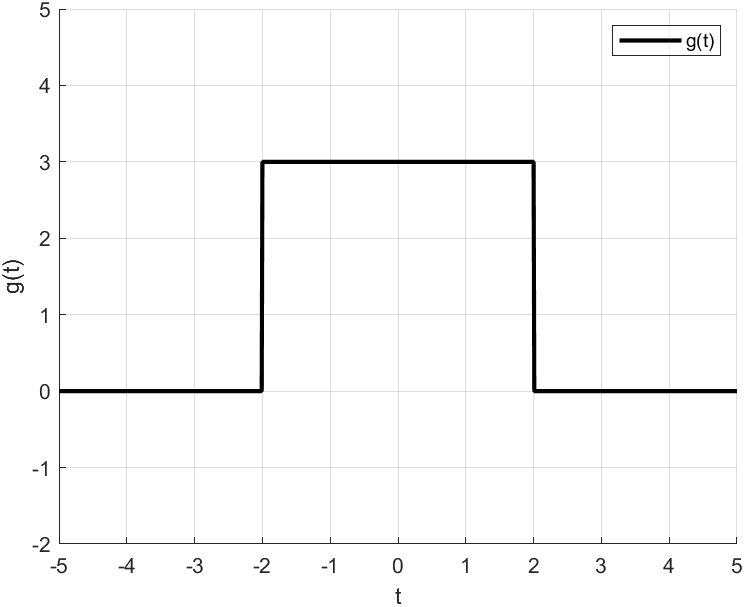
\includegraphics[width=0.5\linewidth]{g(t).png}
    \caption{Исходная функция $g(t)$}
    \label{fig:enter-label}
\end{figure}\

Для моделирования помех при передаче сигнала используется функция $u(t) = g(t) + b\,\xi(t) + c \sin{(dt)}$, где $\xi(t)$ --- равномерное распределение, а $b,c,d$ являются параметрами возмущения. И моей задачей в этой работе является восстановление $g(t)$ из зашумлённой $u(t)$, для выполнения этой задачи необходимо выполнить фильтрацию сигнала с помехами.\ 

Для проведения такой фильтрации сигнала от шумов необходимо построить амплитуду Фурье-образа сигнала с шумами, наложить фильтр для отсеивания лишних частот, которые и являются помехами (чаще всего высокочастотными), а затем выполнить обратное преобразование Фурье, чтобы от образа перейти к исходному сигналу, в результате получится сигнал, близкий к изначальному $g(t)$, но лишённый отсеянных частот.

\subsection{Обработка высоких частот}\

В этом пункте в $u(t)$ нет составляющей, отвечающей за колебательный шум $(c = 0)$, а значит, в каждой точке графика исходная функция будет смещена вверх или вниз, что на графике Фурье-образа будет отвечать за наличие ненулевых значений, соответствующих высоким по модулю частотам (высокочастотные шумы). Коэффициенты $b$ я буду рассматривать из следующего набора: $[0.5, 1, 3]$. Для каждого значения $b$ были подобраны $\nu_0$, при которых отфильтрованная функция лучше всего совпадает с исходной $g(t)$ (проверка осуществлялась путём численного интегрирования разности фильтрованной функции и исходной), получившиеся результаты отображены на графиках.\

Стоит отметить, что в силу случайности значений $\xi(t)$ тяжело найти какое-то наиболее подходящее $\nu_0$ (понимаю, что это не требовалось), так как если, к примеру, при $\nu_0=0.5$ функции совпадают довольно близко, а на соседних рассматриваемых значениях $0.4$ и $0.6$ разница между исходным сигналом и фильтрованным больше, чем в том, что между ними, то вовсе не факт, что $\nu_0=0.5$ лучшее значение --- в $\nu_0=0.7$ разница между функциями может быть меньше. Иными словами, функция разницы между фильтрованной функцией и исходной от выбранного $\nu_0$ частот не унимодальна.\\

Для первого значения $b=0.5$ лучшим диапазоном частот оказался $[-5.4, 5.4]$:

\begin{figure}[H]
    \begin{minipage}{0.5\textwidth}
        \centering
        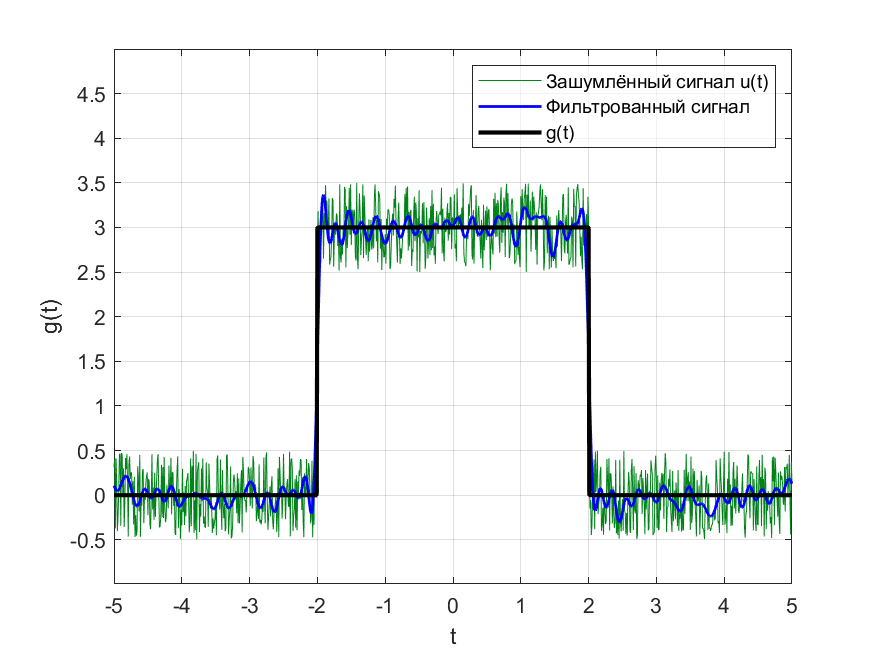
\includegraphics[width=\textwidth]{part1/0.5_5.4.png}
        \caption{$b=0.5, \nu_0 = 5.4$}
    \end{minipage}    
    \begin{minipage}{0.5\textwidth}
        \centering
        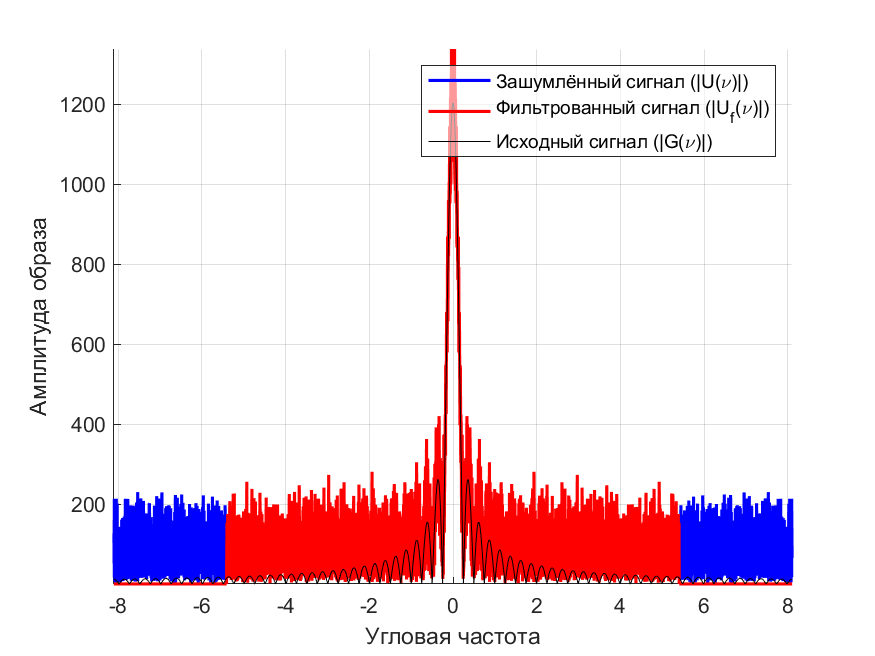
\includegraphics[width=\textwidth]{part1/0.5_5.4_Fourier.png}
        \caption{Модуль Фурье-образа при $b=0.5, \nu_0 = 5.4$}
    \end{minipage}
\end{figure}\ 

При $b = 0.5$ шумы относительно небольшие, самым оптимальным подобранным $\nu_0$ оказалось $\nu_0=5.4$. При $\nu_0 \in (0, 5.4)$ будет взято гораздо меньше полезных частот, не являющихся шумами, но отфильтрованная функция всё ещё будет похожа на изначальную, при этом чем меньший промежуток Фурье-образа будет взят на рассмотрение, тем больше будут периоды колебаний в отфильтрованной функции, что аналогично взятию малого числа коэффициентов в разложении Фурье.\ 

И напротив, выбор $\nu_0$ сильно больших чем оптимальный даёт помехи сравнимые с теми, что создаются слагаемым $b \, \xi(t)$. Случай $\nu_0 = 0$ рассматривать не имеет смысла, так как в этом случае получается, что длина рассматриваемого диапазона частот будет равняться $0$, очевидно что в этом случае фильтрованная функция будет равняться нулю на всей области своего определения, какой бы она ни была.\ 

Такие ``неоптимальные'' случаи выбора $\nu_0$ продемонстрирую для $b = 0.5$, дальше они будут опущены, так как мало что поменяется при выборе других $b$:

\begin{figure}[H]
    \begin{minipage}{0.5\textwidth}
        \centering
        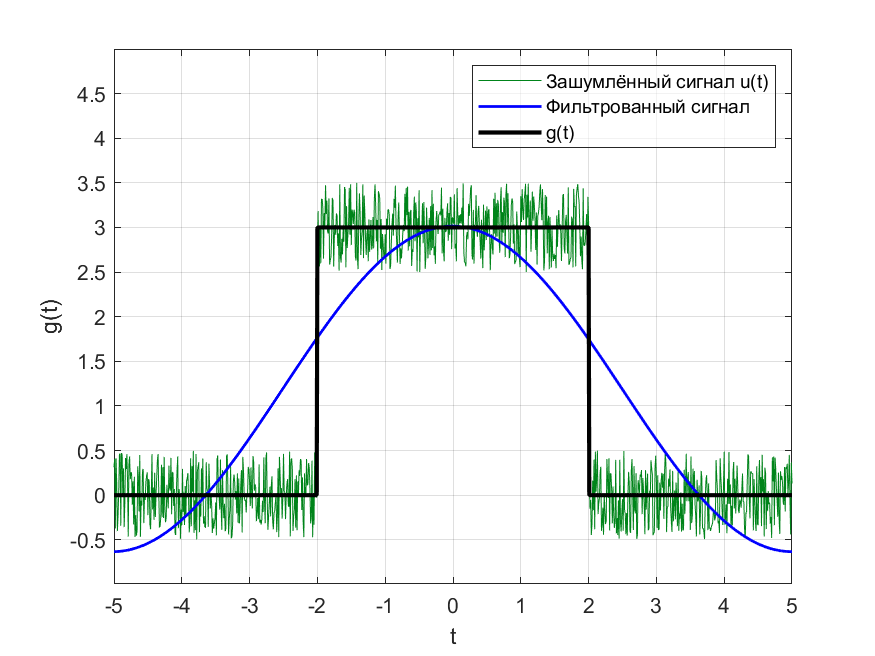
\includegraphics[width=\textwidth]{part1/0.5_0.1.png}
        \caption{$b=0.5, \nu_0 = 0.1$}
    \end{minipage}    
    \begin{minipage}{0.5\textwidth}
        \centering
        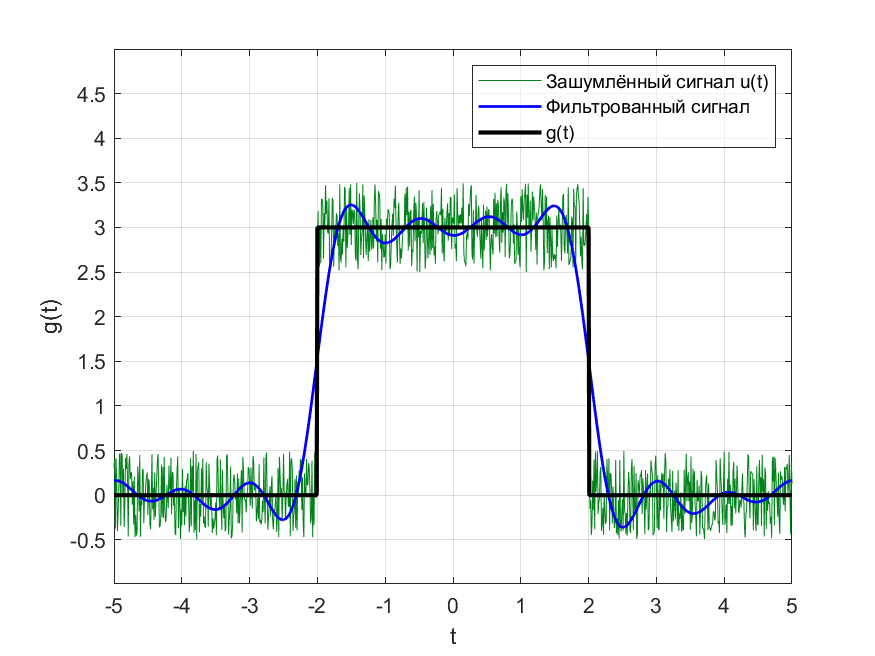
\includegraphics[width=\textwidth]{part1/0.5_1.png}
        \caption{$b=0.5, \nu_0 = 1$}
    \end{minipage}
\end{figure}\ 

\begin{figure}[H]
    \begin{minipage}{0.5\textwidth}
        \centering
        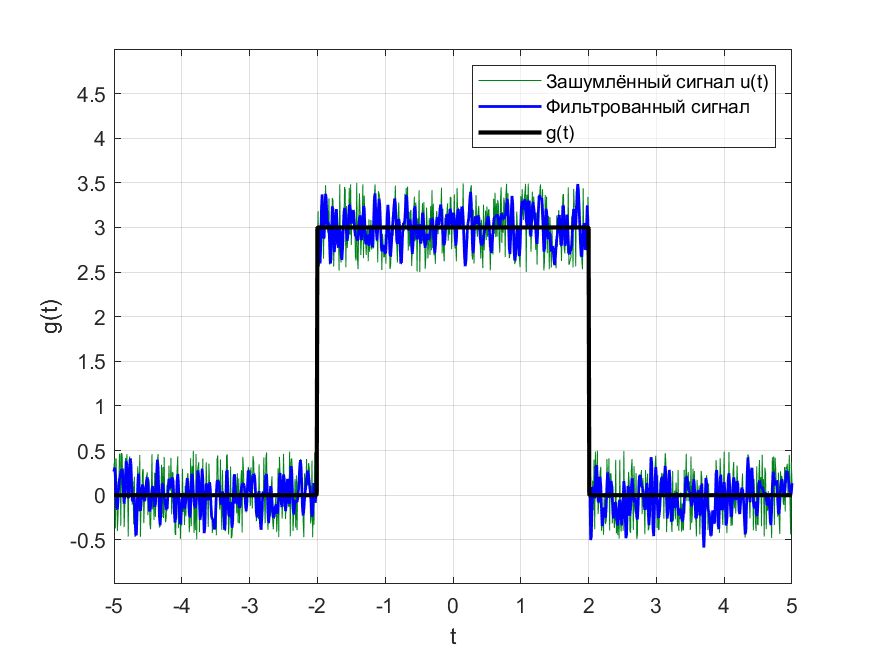
\includegraphics[width=\textwidth]{part1/0.5_20.png}
        \caption{$b=0.5, \nu_0 = 20$}
    \end{minipage}    
    \begin{minipage}{0.5\textwidth}
        \centering
        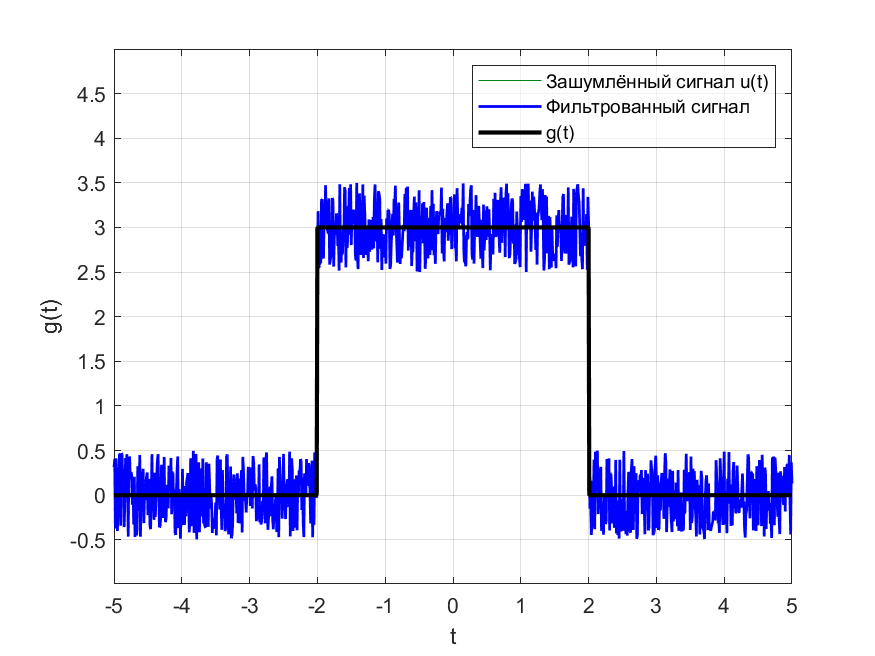
\includegraphics[width=\textwidth]{part1/0.5_200.png}
        \caption{$b=0.5, \nu_0 = 50$}
    \end{minipage}
\end{figure}\ 

Графики модулей Фурье-образов для этих случаев:

\begin{figure}[H]
    \begin{minipage}{0.5\textwidth}
        \centering
        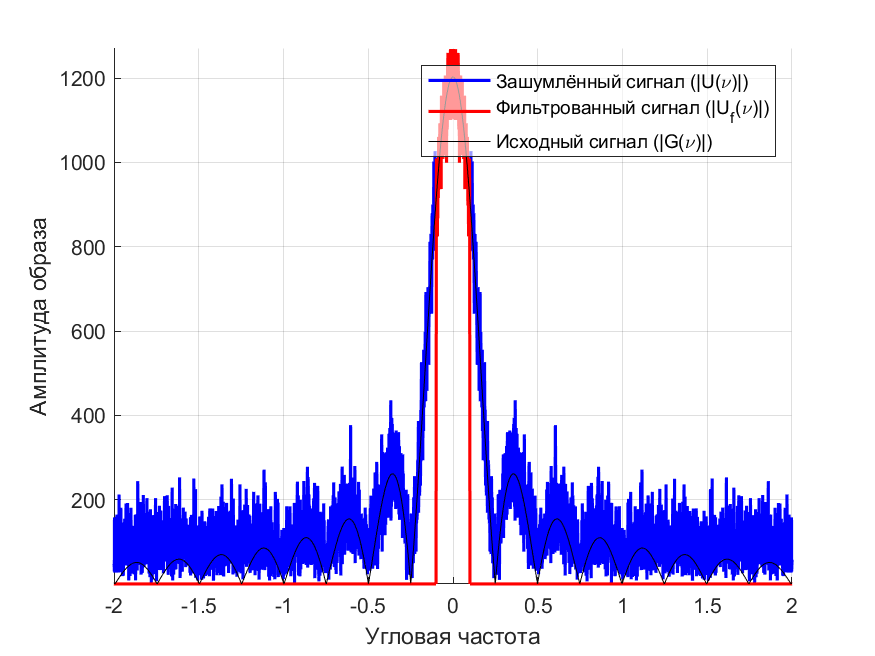
\includegraphics[width=\textwidth]{part1/0.5_0.1_Fourier.png}
        \caption{$b=0.5, \nu_0 = 0.1$}
    \end{minipage}    
    \begin{minipage}{0.5\textwidth}
        \centering
        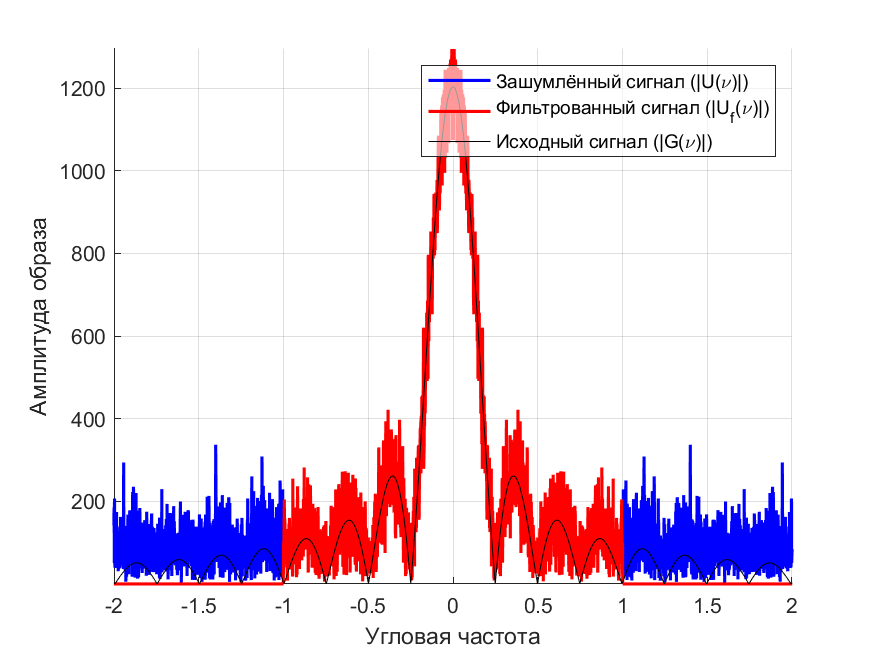
\includegraphics[width=\textwidth]{part1/0.5_1_Fourier.png}
        \caption{$b=0.5, \nu_0 = 1$}
    \end{minipage}
\end{figure}\ 

\begin{figure}[H]
    \begin{minipage}{0.5\textwidth}
        \centering
        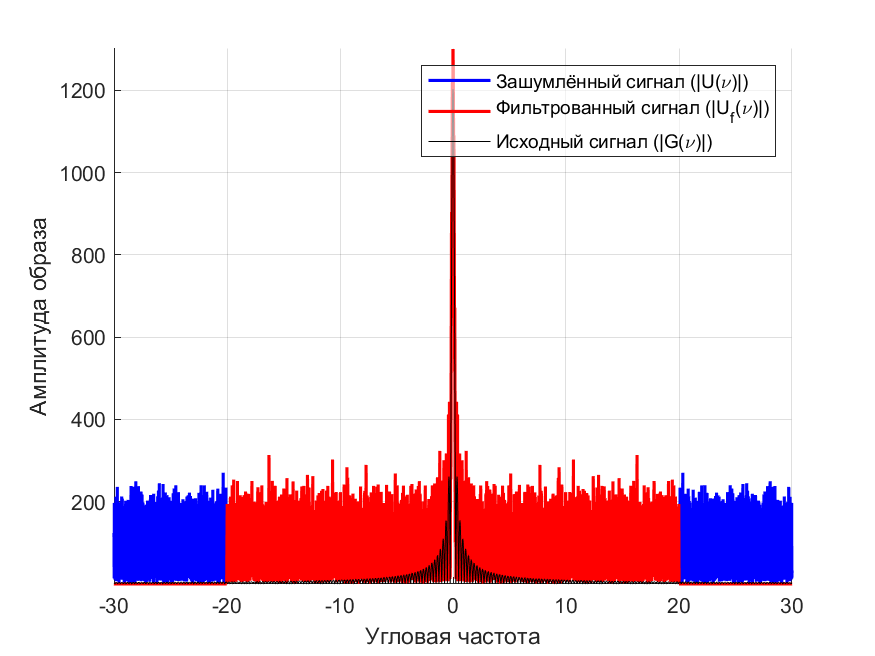
\includegraphics[width=\textwidth]{part1/0.5_20_Fourier.png}
        \caption{$b=0.5, \nu_0 = 20$}
    \end{minipage}    
    \begin{minipage}{0.5\textwidth}
        \centering
        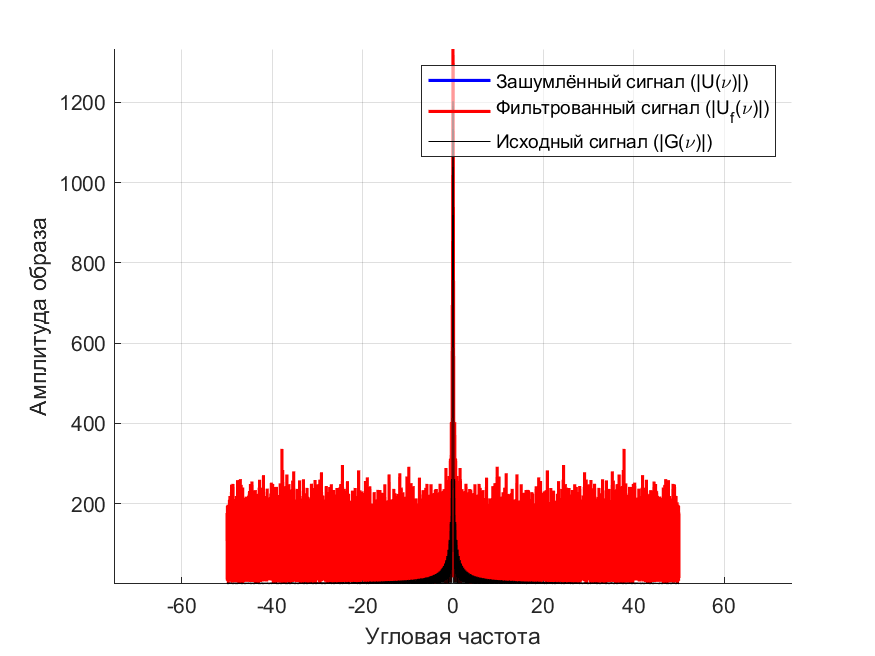
\includegraphics[width=\textwidth]{part1/0.5_50_Fourier.png}
        \caption{$b=0.5, \nu_0 = 50$}
    \end{minipage}
\end{figure}\ 

Для $b = 1$ наиболее оптимальным оказался $\nu_0=4.4$:

\begin{figure}[H]
    \begin{minipage}{0.5\textwidth}
        \centering
        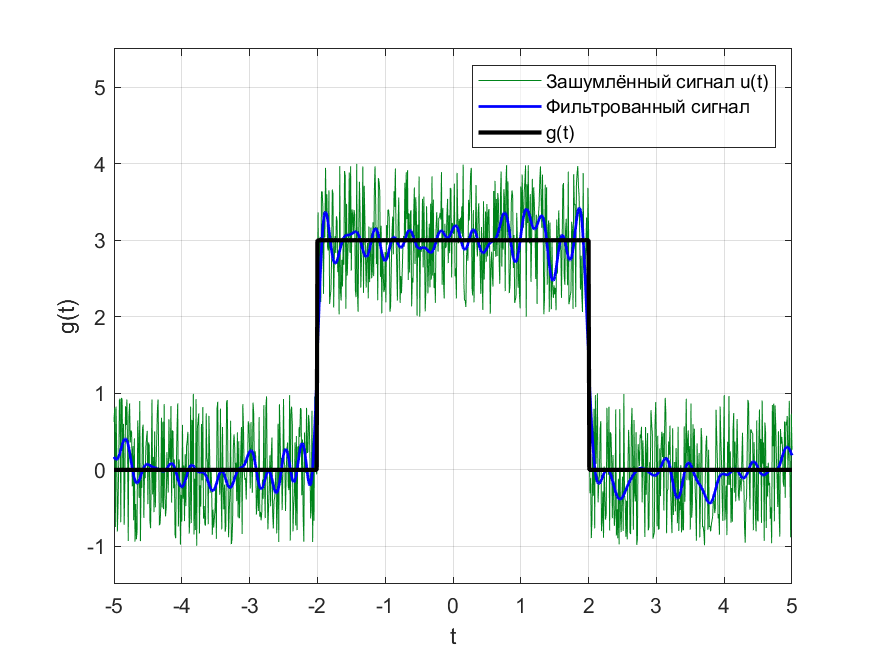
\includegraphics[width=\textwidth]{part1/1_4.4.png}
        \caption{$b=1, \nu_0 = 4.4$}
    \end{minipage}    
    \begin{minipage}{0.5\textwidth}
        \centering
        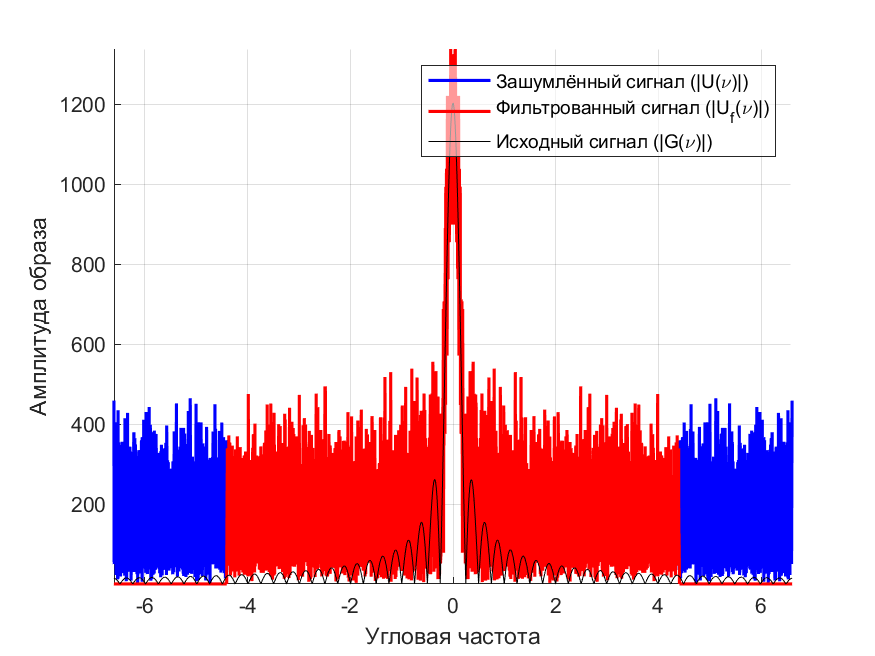
\includegraphics[width=\textwidth]{part1/1_4.4_Fourier.png}
        \caption{Модуль Фурье-образа, $b=1, \nu_0 = 4.4$}
    \end{minipage}
\end{figure}\

Для $b = 3$ же получаем следующий результат:

\begin{figure}[H]
    \begin{minipage}{0.5\textwidth}
        \centering
        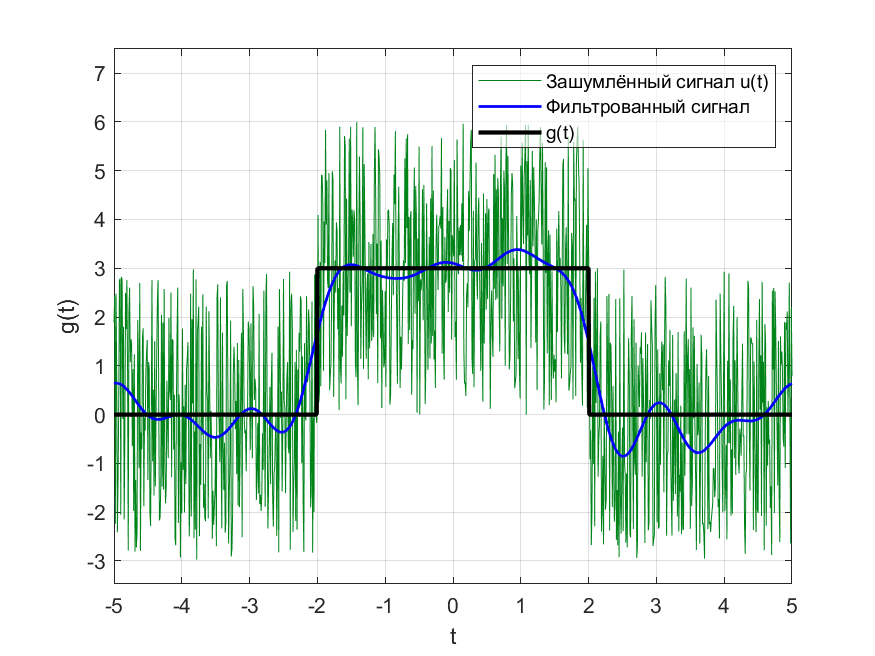
\includegraphics[width=\textwidth]{part1/3_1.png}
        \caption{$b=3, \nu_0 = 1$}
    \end{minipage}    
    \begin{minipage}{0.5\textwidth}
        \centering
        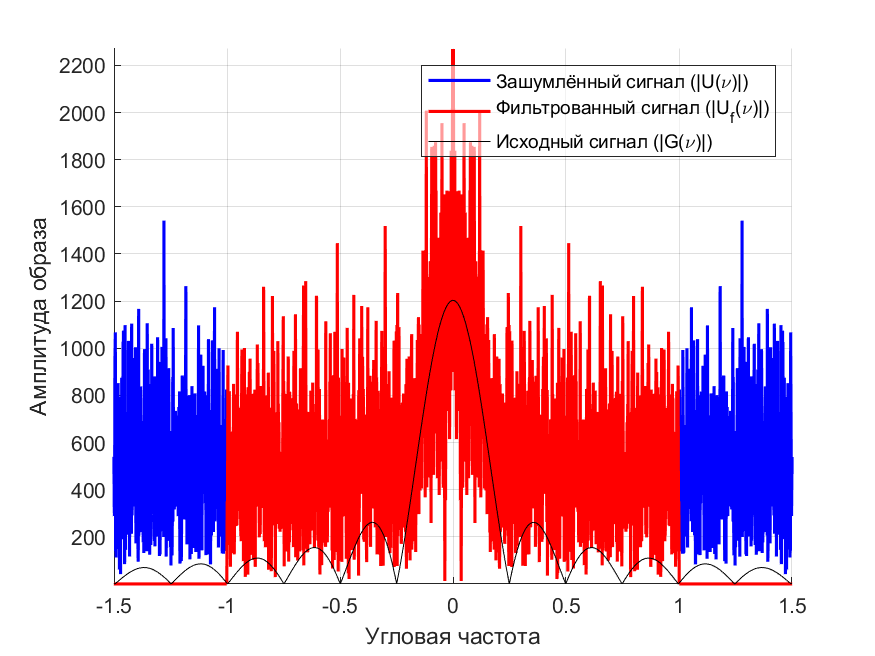
\includegraphics[width=\textwidth]{part1/3_1_Fourier.png}
        \caption{Модуль Фурье-образа, $b=3, \nu_0 = 1$}
    \end{minipage}
\end{figure}\

В этом же случае помехи очень большие. Если при предыдущих значениях $b$ интеграл модуля разницы функций давал при лучших значениях $1.39$ при $b = 1$ и $0.81$ при $b = 0.5$, то сейчас минимальное значение, которого удалось достичь --- $2.36$ с сохранённым диапазоном частот $[-1, 1]$, а значит, полезный сигнал был утерян в большей степени, чем раньше (так будет происходить и дальше по мере роста $b$).\\

Теперь то же самое, но с фиксированным $\nu_0$. В этом случае будет взято только одно значение --- $\nu_0 = 3$.\

При $b = 10^{-10}$ фильтрованный сигнал получается очень похож на обычное приближение рядом Фурье с небольшим числом базисных функций:

\begin{figure}[H]
    \begin{minipage}{0.5\textwidth}
        \centering
        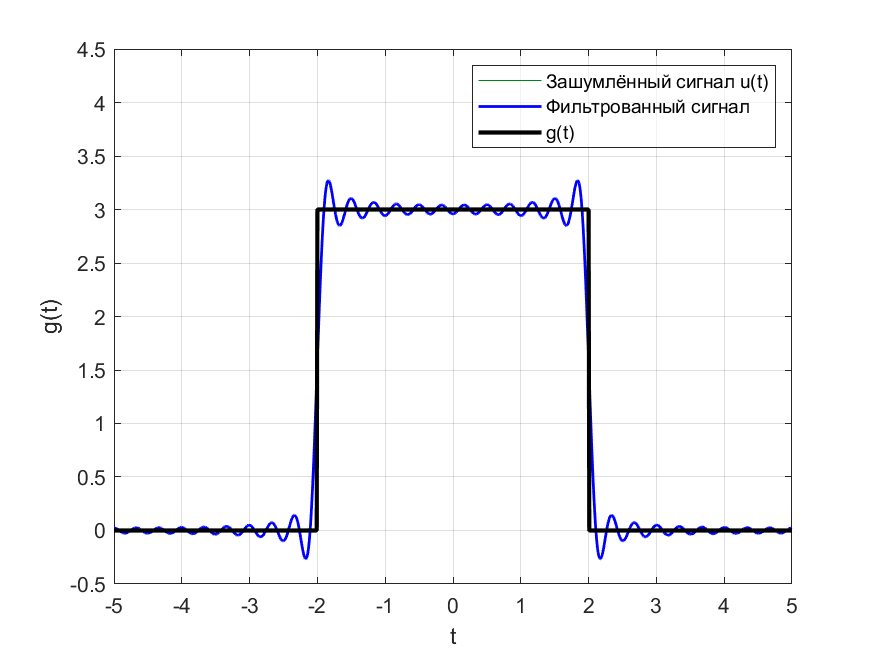
\includegraphics[width=\textwidth]{part1/1e-10_3.png}
        \caption{$b=10^{-10}, \nu_0 = 3$}
    \end{minipage}    
    \begin{minipage}{0.5\textwidth}
        \centering
        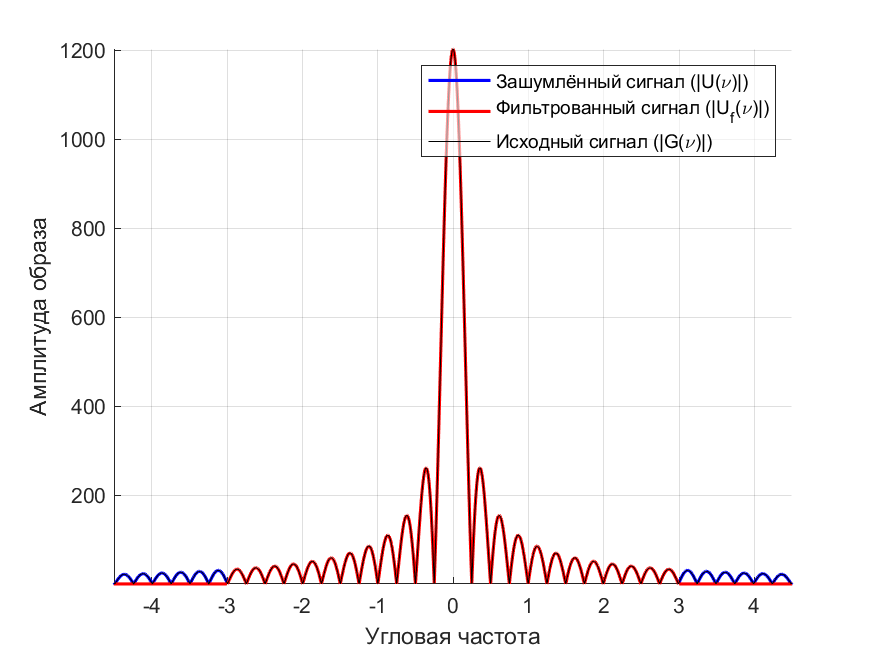
\includegraphics[width=\textwidth]{part1/1e-10_3_Fourier.png}
        \caption{Модуль Фурье-образа, $b=10^{-10}, \nu_0 = 3$}
    \end{minipage}
\end{figure}\

При $b = 0.5$ не всё так идеально, но видно, что функция приближается к исходной:

\begin{figure}[H]
    \begin{minipage}{0.5\textwidth}
        \centering
        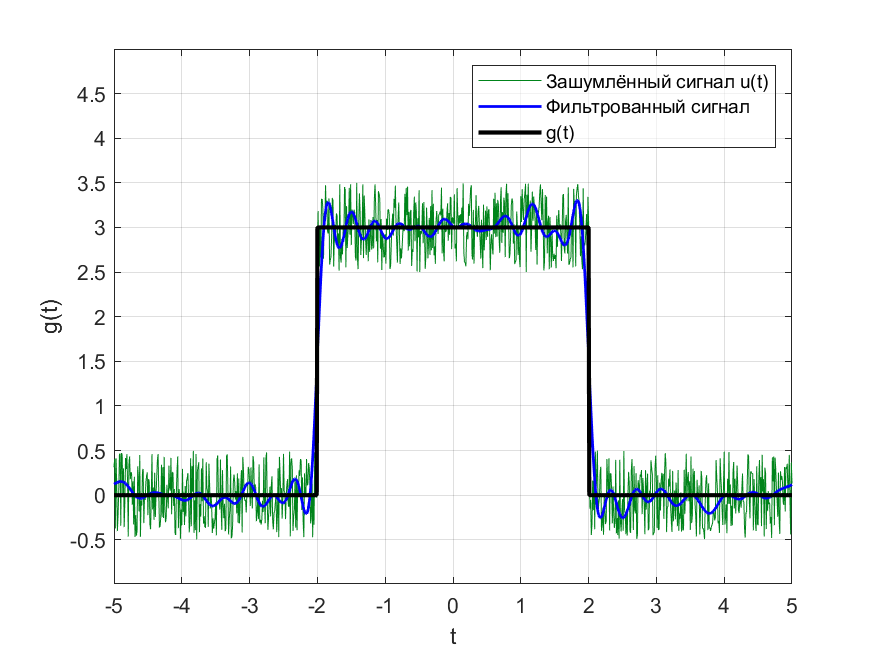
\includegraphics[width=\textwidth]{part1/0.5_3.png}
        \caption{$b=0.5, \nu_0 = 3$}
    \end{minipage}    
    \begin{minipage}{0.5\textwidth}
        \centering
        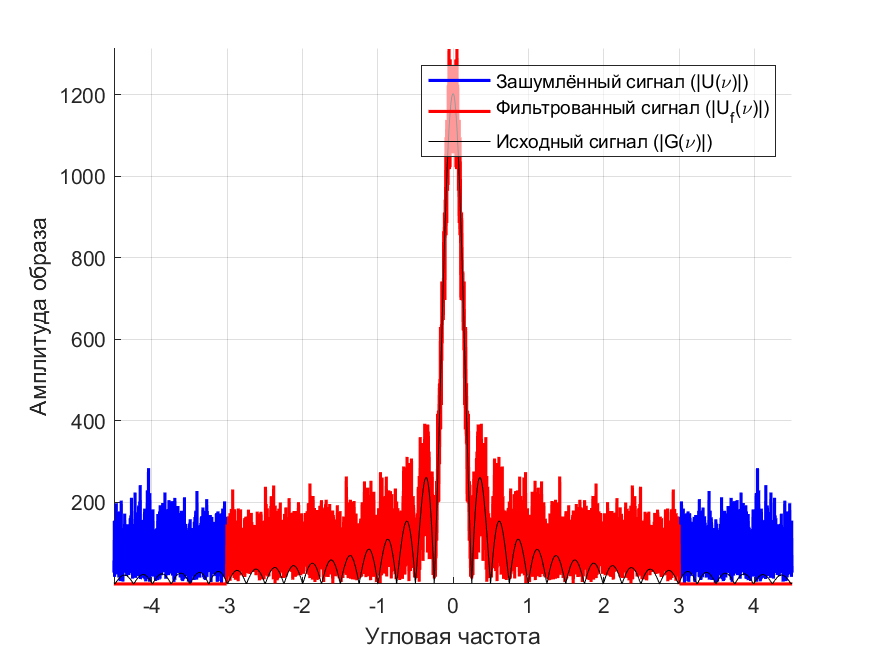
\includegraphics[width=\textwidth]{part1/0.5_3_Fourier.png}
        \caption{Модуль Фурье-образа, $b=0.5, \nu_0 = 3$}
    \end{minipage}
\end{figure}\

При $b = 3$ всё ещё можно понять очертания исходной функции:

\begin{figure}[H]
    \begin{minipage}{0.5\textwidth}
        \centering
        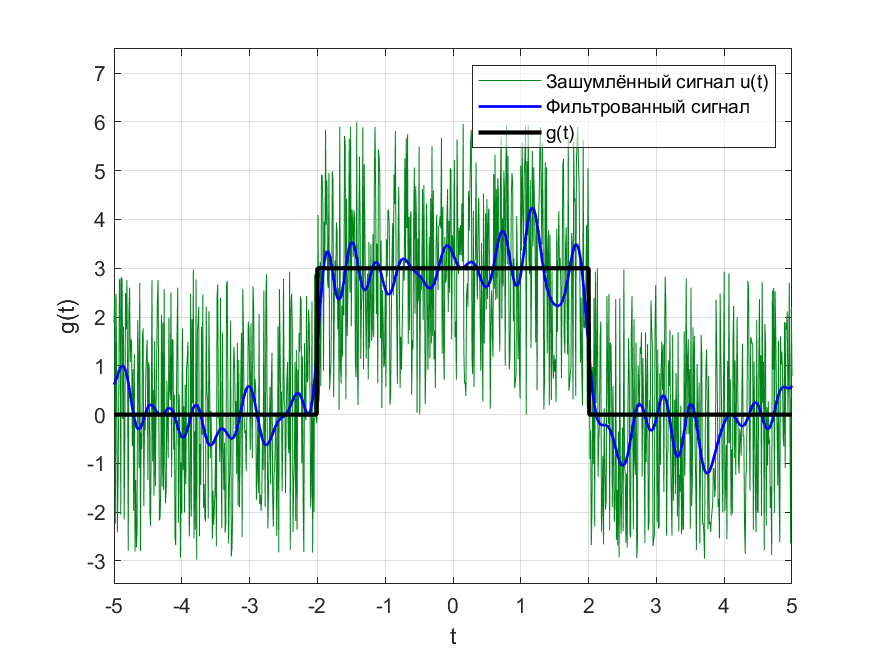
\includegraphics[width=\textwidth]{part1/3_3.png}
        \caption{$b=3, \nu_0 = 3$}
    \end{minipage}    
    \begin{minipage}{0.5\textwidth}
        \centering
        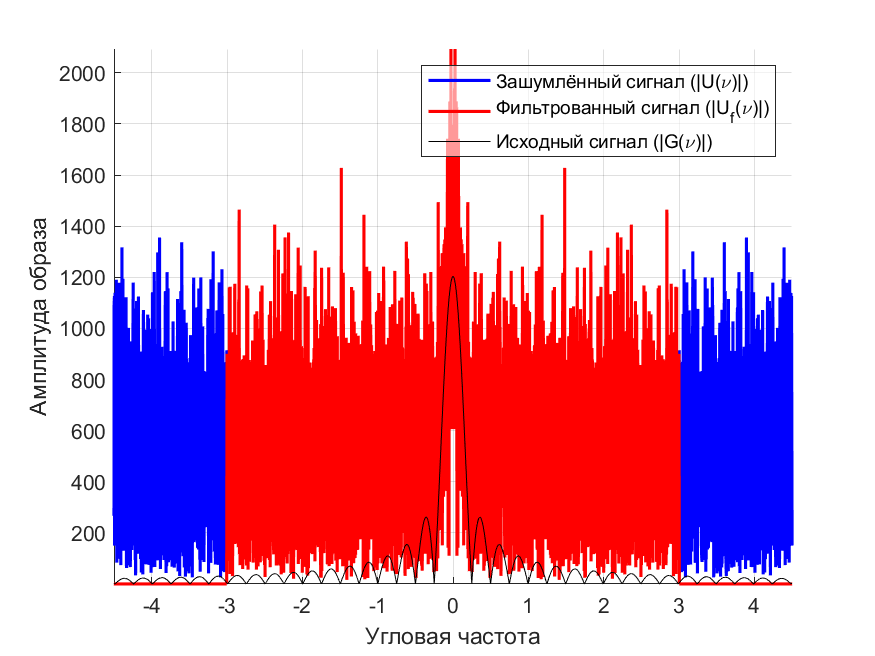
\includegraphics[width=\textwidth]{part1/3_3_Fourier.png}
        \caption{Модуль Фурье-образа, $b=3, \nu_0 = 3$}
    \end{minipage}
\end{figure}\

А вот при $b = 10$ становится немного печально:

\begin{figure}[H]
    \begin{minipage}{0.5\textwidth}
        \centering
        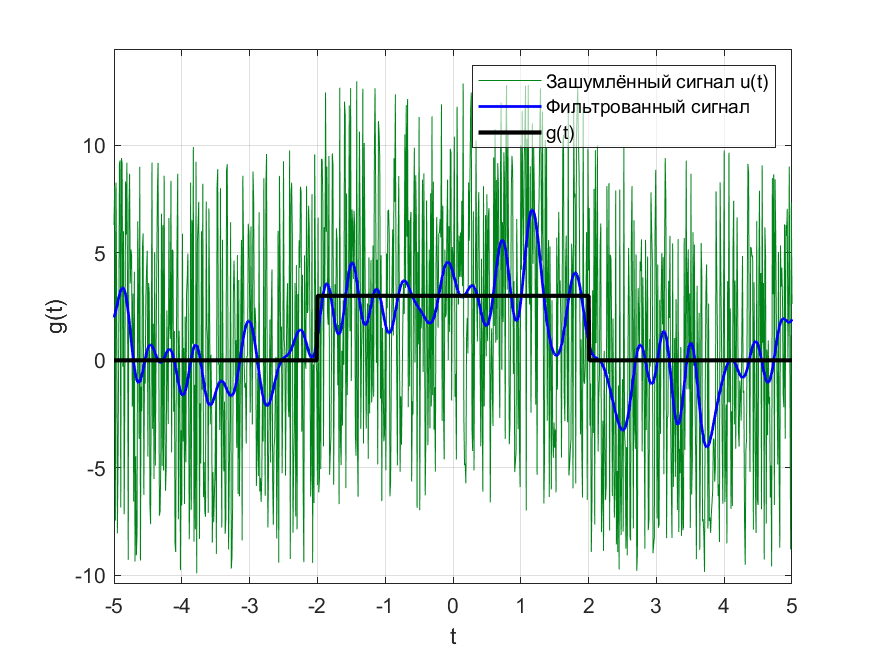
\includegraphics[width=\textwidth]{part1/10_3.png}
        \caption{$b=10, \nu_0 = 3$}
    \end{minipage}    
    \begin{minipage}{0.5\textwidth}
        \centering
        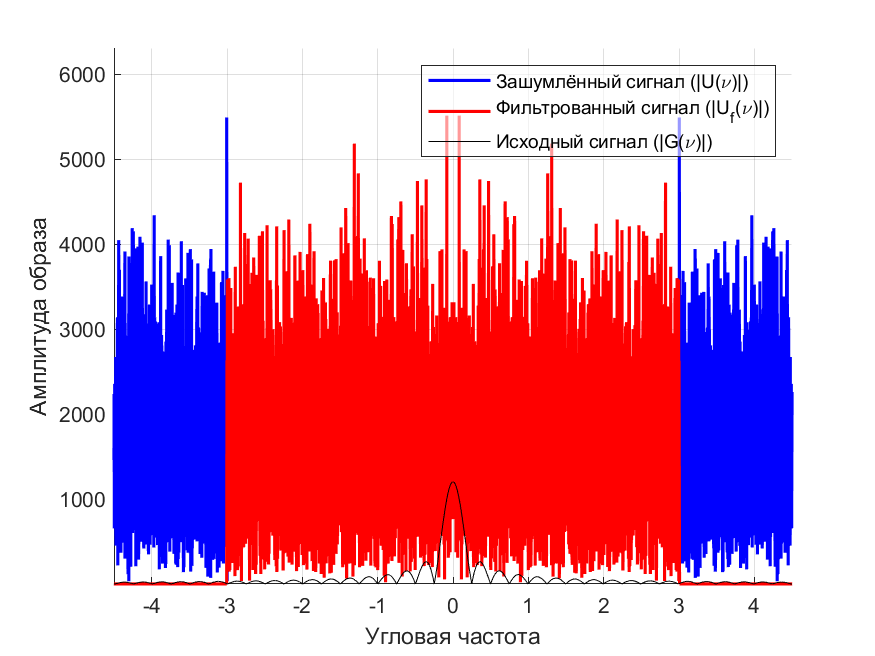
\includegraphics[width=\textwidth]{part1/10_3_Fourier.png}
        \caption{Модуль Фурье-образа, $b=10, \nu_0 = 3$}
    \end{minipage}
\end{figure}\

Видно, что в этом случае отклонения фильтрованной функции от исходной превышают её значение, что позволяет сделать вывод о том, что при подобных помехах значительная часть сигнала неизбежно потеряется.

\subsubsection{Вывод}\

Теперь я понимаю, как именно коэффициент $b$ влияет на помехи, и что при больших $b$ эффективность фильтрации ниже, чем при малых, а также что слишком большие, как и слишком малые $\nu_0$ не есть хорошо, ибо фильтрация в таком случае теряет свой смысл (берётся слишком мало исходных данных или, наоборот, настолько много, что помехи почти не отсеиваются)

\subsection{Обработка специфических частот}\

В этом пункте к белому шуму $b \, \xi (t)$ добавляются гармонические помехи $c \, \sin{(dt)}$. На графике Фурье-образа они дают резкие скачки на некоторых частотах, симметричных относительно начала координат (разумеется, ведь модуль образа Фурье --- функция четная), и, помимо применения фильтра нижних частот, теперь нужно будет обнулить эти скачки, чтобы убрать влияние гармонических помех.\

Начну с выбора коэффициентов, в этот раз буду использовать стандартный набор, и поочерёдно изменять каждый из них, наблюдая, как меняется при этом функция: $b = 1, c = 1, d = 1$. Частота среза же изначально будет равна $5$.\ 

Вот как это будет выглядеть в стандартном случае:

\begin{figure}[H]
    \begin{minipage}{0.5\textwidth}
        \centering
        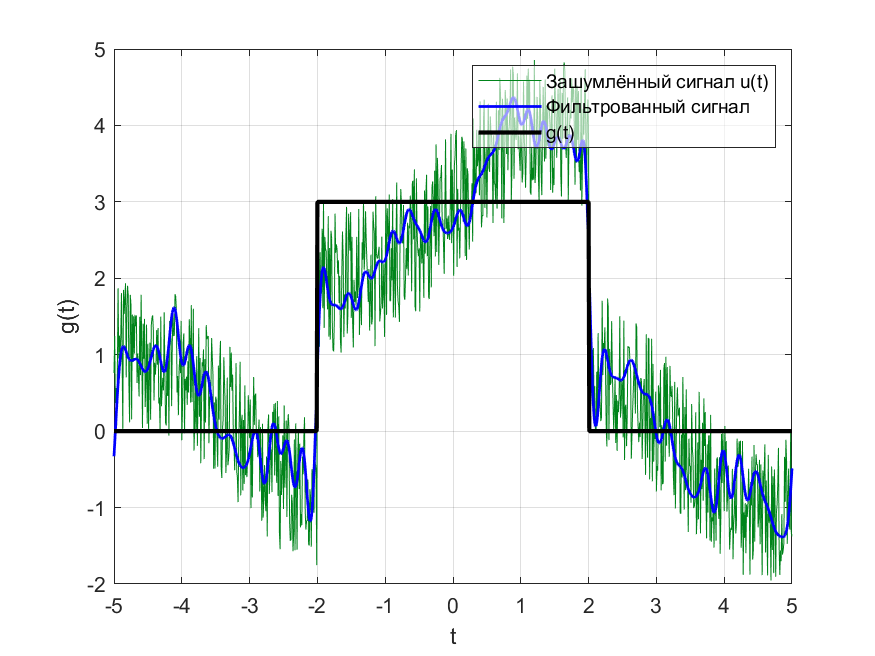
\includegraphics[width=\textwidth]{part2/1_1_1.png}
        \caption{$b = 1, c = 1, d = 1, \nu_0 = 5$}
    \end{minipage}    
    \begin{minipage}{0.5\textwidth}
        \centering
        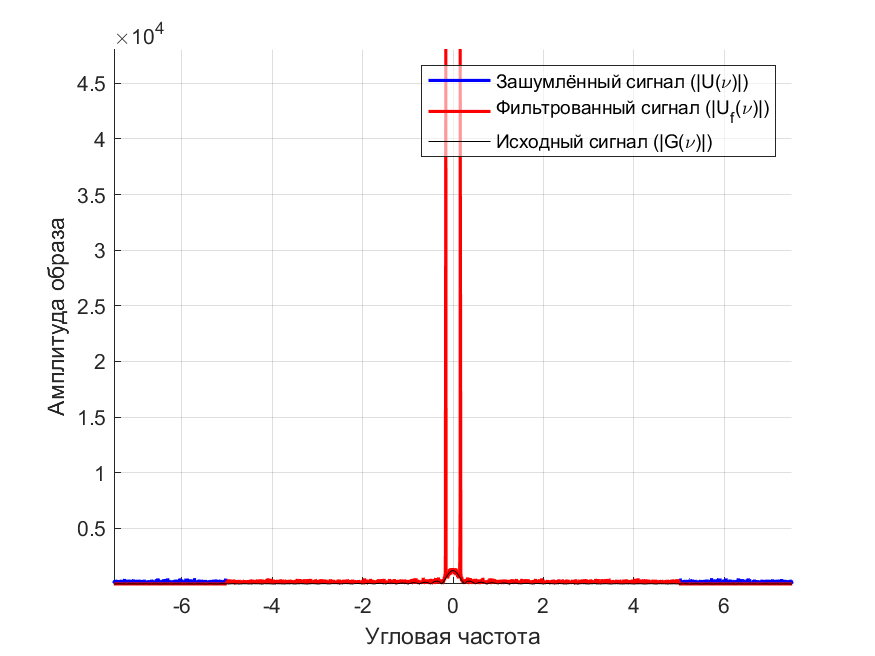
\includegraphics[width=\textwidth]{part2/1_1_1_Fourier.png}
        \caption{Модуль Фурье-образа, $b = 1, c = 1, d = 1, \nu_0 = 5$}
    \end{minipage}
\end{figure}\

\begin{figure}[H]
    \centering
    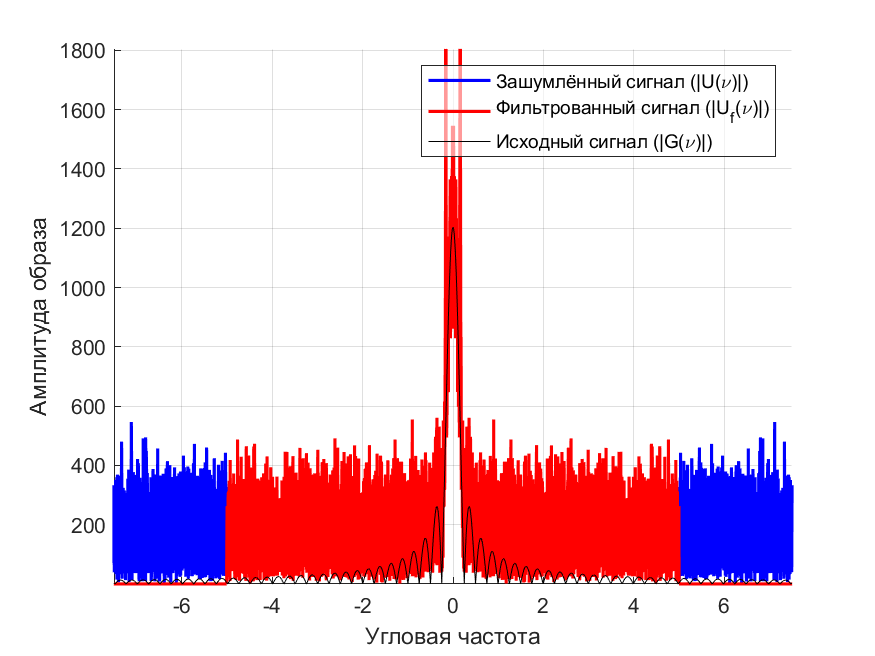
\includegraphics[width=0.5\linewidth]{part2/1_1_1_Fourier_scaled.png}
    \caption{Модуль Фурье-образа в приближении, $b = 1, c = 1, d = 1, \nu_0 = 5$}
\end{figure}\

\subsubsection{Исследование влияния значения параметра $b$}

Исследуем влияние параметра $b$ на вид помехи и эффективность фильтрации. При $b = 0$:

\begin{figure}[H]
    \begin{minipage}{0.5\textwidth}
        \centering
        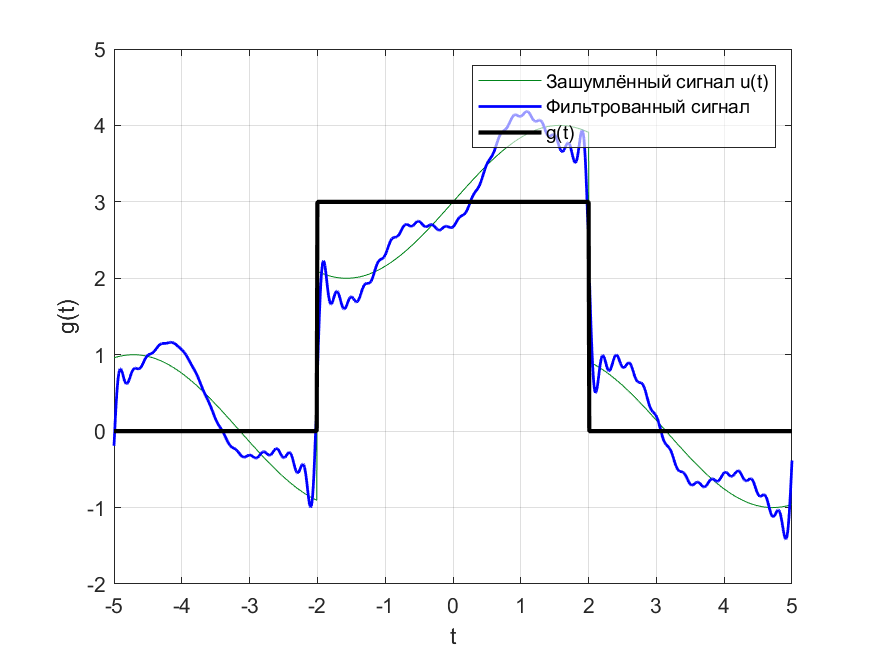
\includegraphics[width=\textwidth]{part2/0_1_1.png}
        \caption{$b = 0, c = 1, d = 1, \nu_0 = 5$}
    \end{minipage}    
    \begin{minipage}{0.5\textwidth}
        \centering
        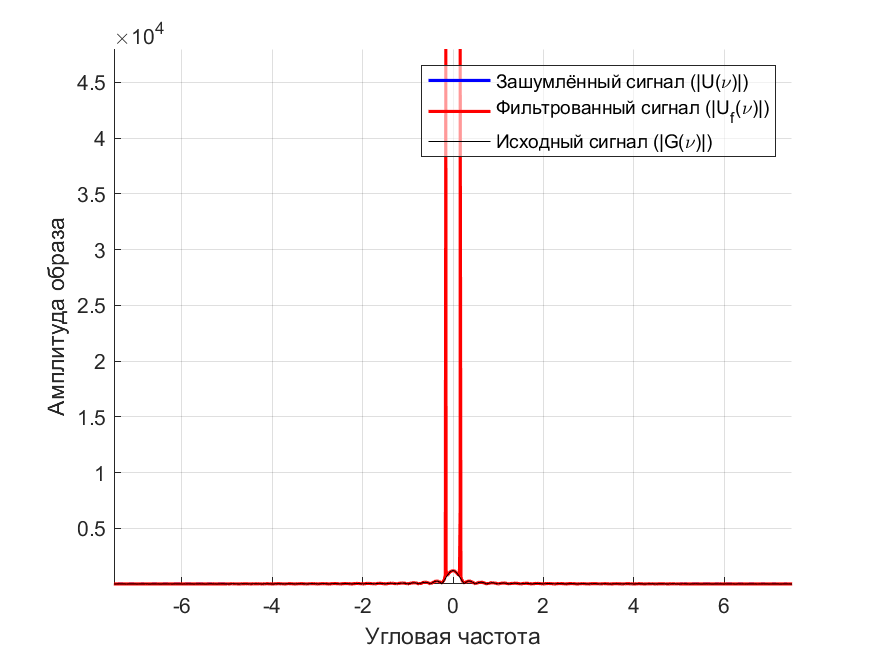
\includegraphics[width=\textwidth]{part2/0_1_1_Fourier.png}
        \caption{Модуль Фурье-образа, $b = 0, c = 1, d = 1, \nu_0 = 5$}
    \end{minipage}
\end{figure}\

\begin{figure}[H]
    \centering
    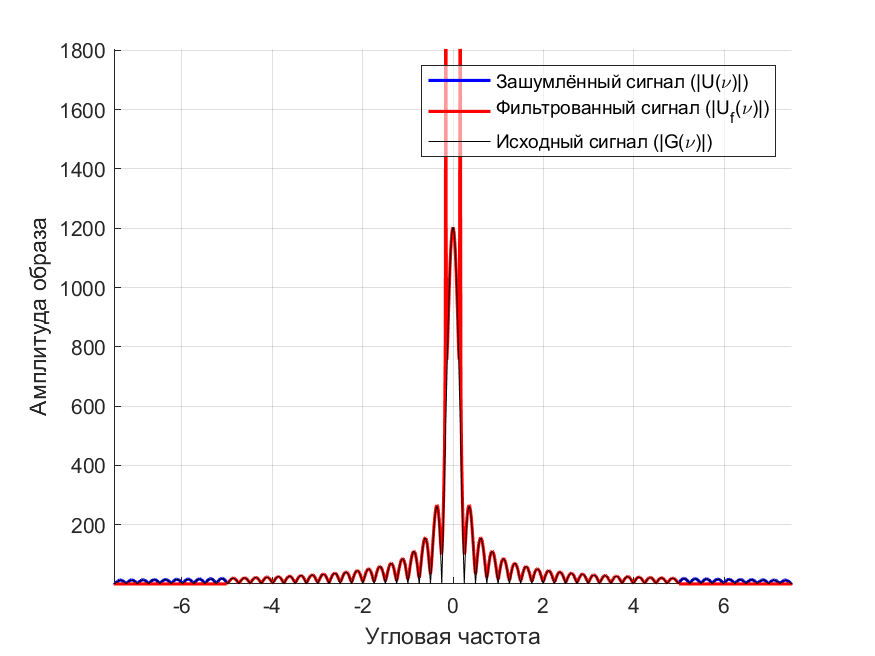
\includegraphics[width=0.5\linewidth]{part2/0_1_1_Fourier_scaled.png}
    \caption{Модуль Фурье-образа в приближении, $b = 0, c = 1, d = 1, \nu_0 = 5$}
\end{figure}\

Видно, что белый шум вовсе пропал, при этом фильтрованный сигнал не в точности повторяет зашумлённый (и не только в местах скачков), хоть тот и представляет собой синусоиду, к которой ряд Фурье сходится довольно быстро.\

При $b = 2$:

\begin{figure}[H]
    \begin{minipage}{0.5\textwidth}
        \centering
        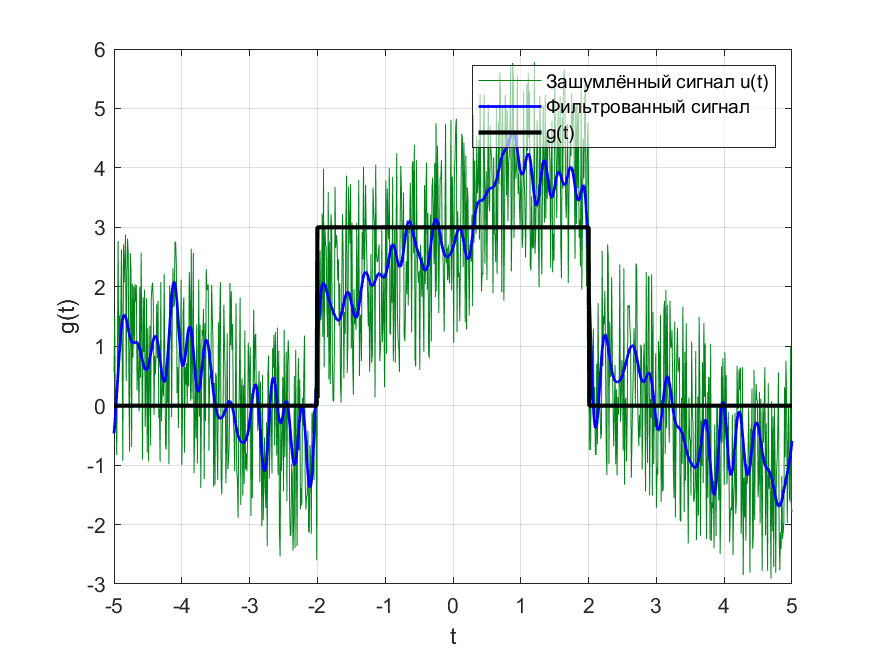
\includegraphics[width=\textwidth]{part2/2_1_1.png}
        \caption{$b = 2, c = 1, d = 1, \nu_0 = 5$}
    \end{minipage}    
    \begin{minipage}{0.5\textwidth}
        \centering
        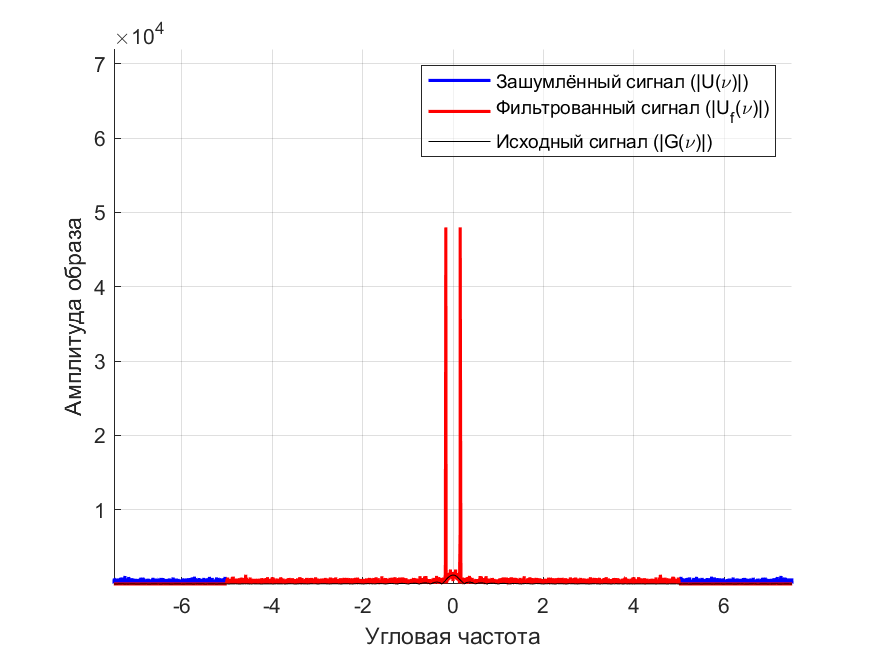
\includegraphics[width=\textwidth]{part2/2_1_1_Fourier.png}
        \caption{Модуль Фурье-образа, $b = 2, c = 1, d = 1, \nu_0 = 5$}
    \end{minipage}
\end{figure}\

\begin{figure}[H]
    \centering
    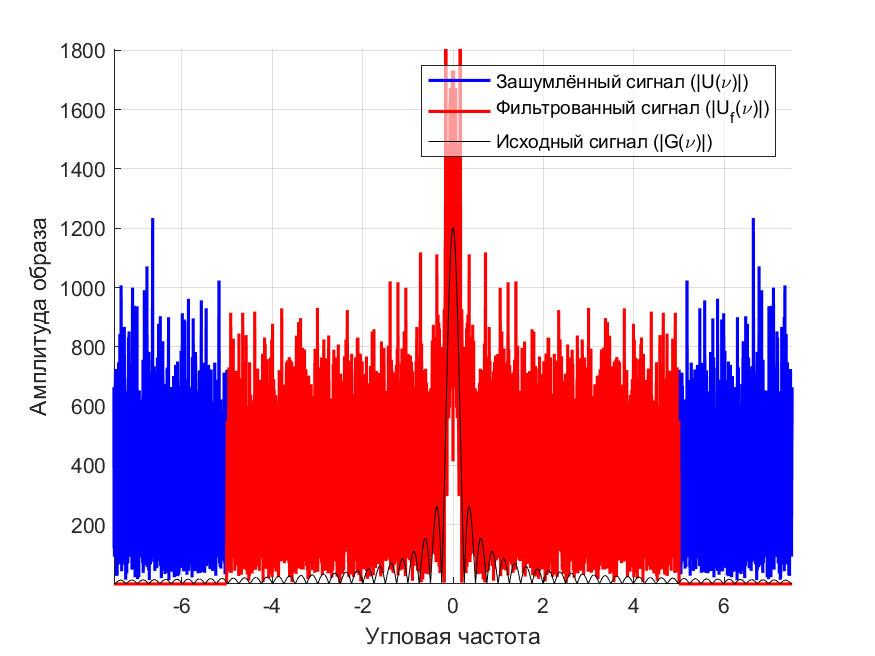
\includegraphics[width=0.5\linewidth]{part2/2_1_1_Fourier_scaled.png}
    \caption{Модуль Фурье-образа в приближении, $b = 2, c = 1, d = 1, \nu_0 = 5$}
\end{figure}\

Отсюда же можно заметить, что амплитуда белого шума заметно увеличилась, а на графике модуля Фурье-образа появились значительные высокочастотные помехи. Можно сделать вывод, что с увеличением $b$ амплитуда таких помех будет увеличиваться, при высоких $b$ фильтрация станет неэффективной.

\subsubsection{Исследование влияния значения параметра $c$}

Случай с $c = 0$ рассмотрен в предыдущем пункте, начнём с $c = 2$:

\begin{figure}[H]
    \begin{minipage}{0.5\textwidth}
        \centering
        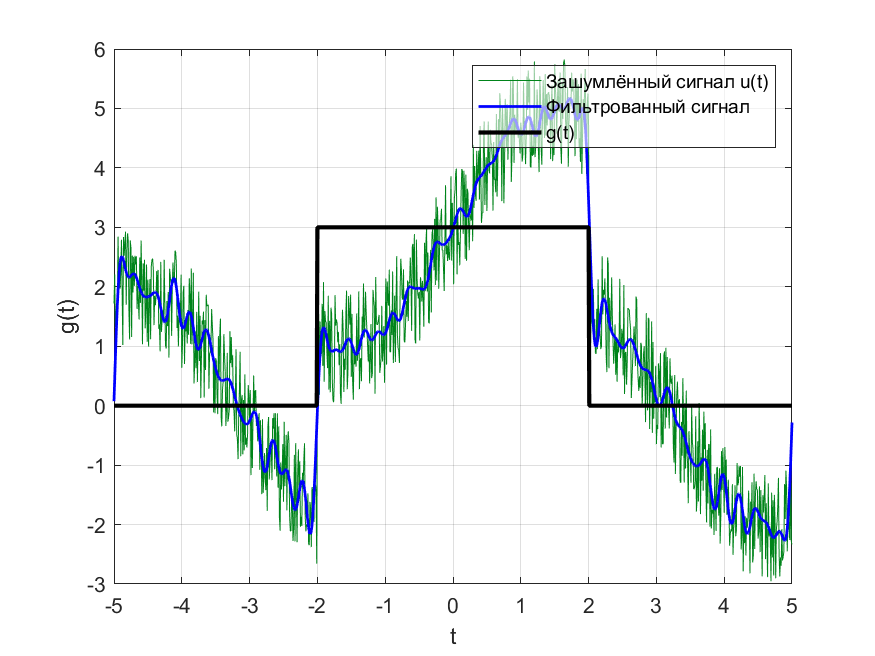
\includegraphics[width=\textwidth]{part2/1_2_1.png}
        \caption{$b = 1, c = 2, d = 1, \nu_0 = 5$}
    \end{minipage}    
    \begin{minipage}{0.5\textwidth}
        \centering
        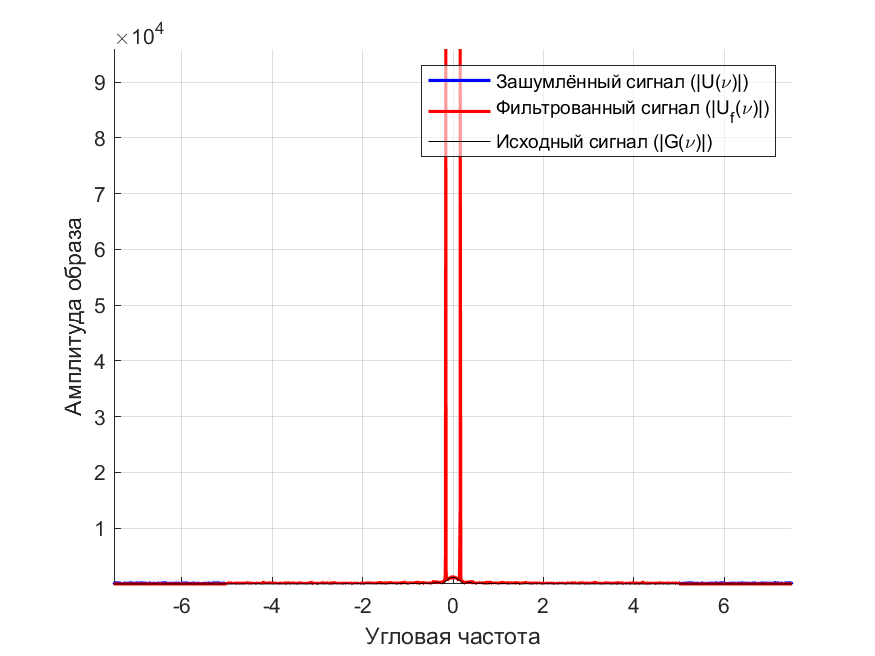
\includegraphics[width=\textwidth]{part2/1_2_1_Fourier.png}
        \caption{Модуль Фурье-образа, $b = 1, c = 2, d = 1, \nu_0 = 5$}
    \end{minipage}
\end{figure}\

\begin{figure}[H]
    \centering
    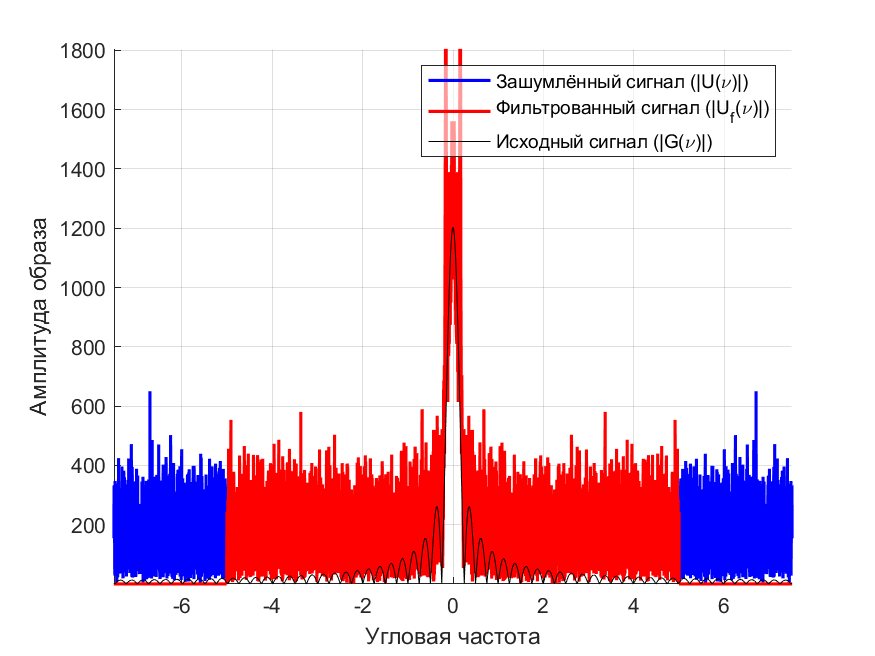
\includegraphics[width=0.5\linewidth]{part2/1_2_1_Fourier_scaled.png}
    \caption{Модуль Фурье-образа в приближении, $b = 1, c = 2, d = 1, \nu_0 = 5$}
\end{figure}\

При $c = 8$:

\begin{figure}[H]
    \begin{minipage}{0.5\textwidth}
        \centering
        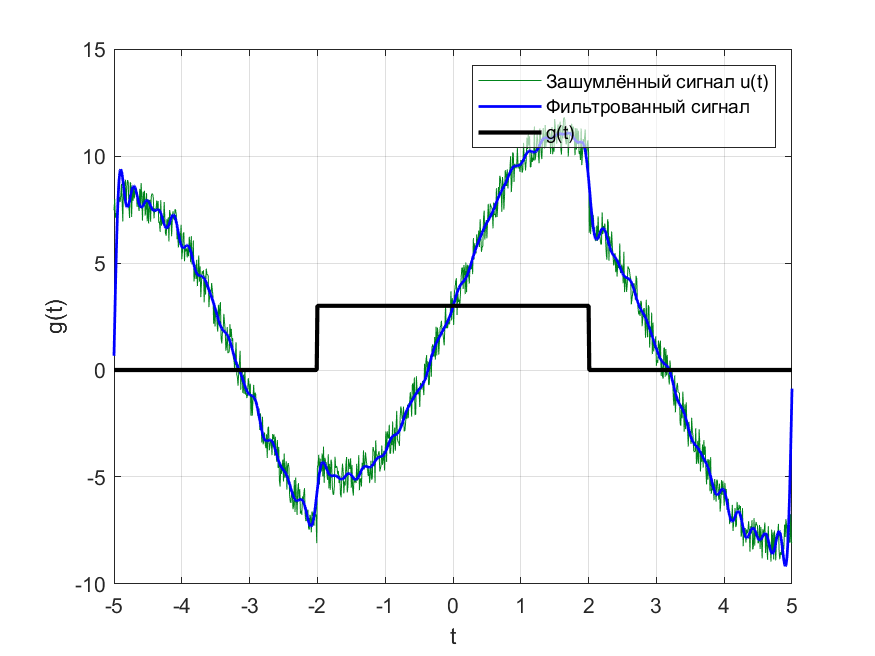
\includegraphics[width=\textwidth]{part2/1_8_1.png}
        \caption{$b = 1, c = 8, d = 1, \nu_0 = 5$}
    \end{minipage}    
    \begin{minipage}{0.5\textwidth}
        \centering
        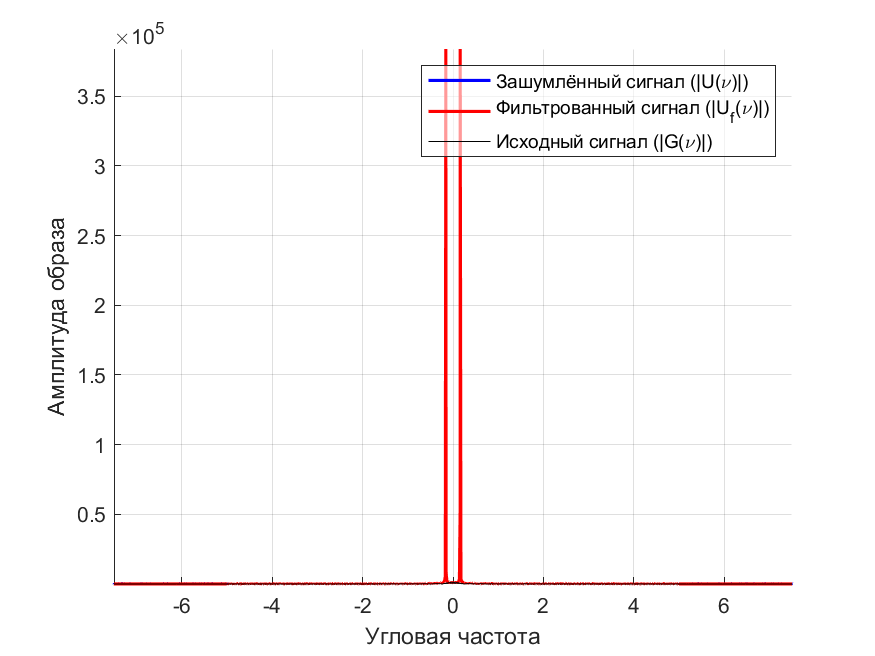
\includegraphics[width=\textwidth]{part2/1_8_1_Fourier.png}
        \caption{Модуль Фурье-образа, $b = 1, c = 8, d = 1, \nu_0 = 5$}
    \end{minipage}
\end{figure}\

\begin{figure}[H]
    \centering
    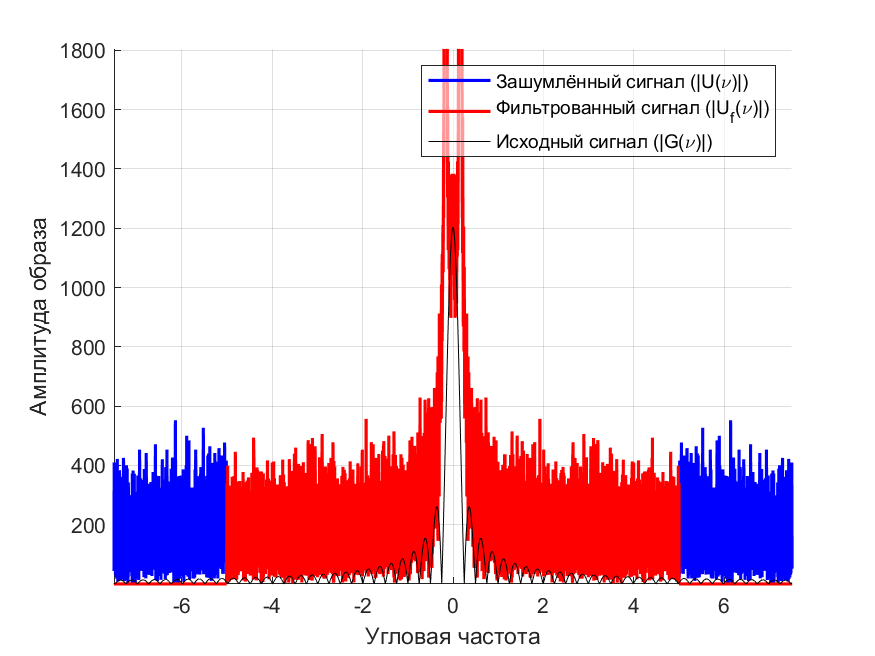
\includegraphics[width=0.5\linewidth]{part2/1_8_1_Fourier_scaled.png}
    \caption{Модуль Фурье-образа в приближении, $b = 1, c = 8, d = 1, \nu_0 = 5$}
\end{figure}\

Из приведённых графиков становится понятно, что меняется амплитуда гармонического шума, и происходит это прямо пропорционально изменению коэффициента $c$. При этом на графиках Фурье-образов заметны пики. Если обнулить амплитуду образа там, где эти пики проявляются, можно получить чуть более приятную картину:

\begin{figure}[H]
    \begin{minipage}{0.5\textwidth}
        \centering
        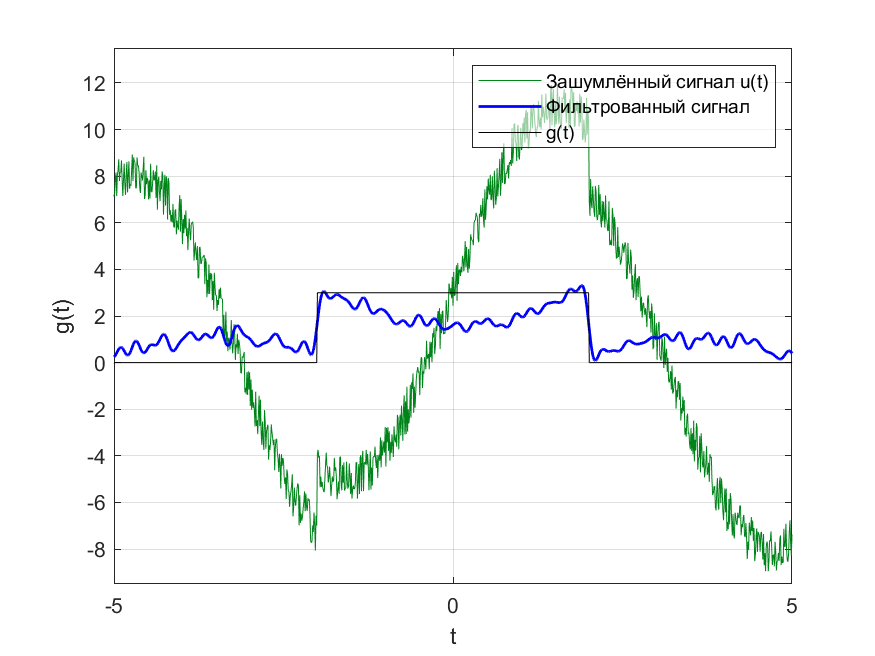
\includegraphics[width=\textwidth]{part2/1_8_1n.png}
        \caption{$b = 1, c = 8, d = 1, \nu_0 = 5$}
    \end{minipage}    
    \begin{minipage}{0.5\textwidth}
        \centering
        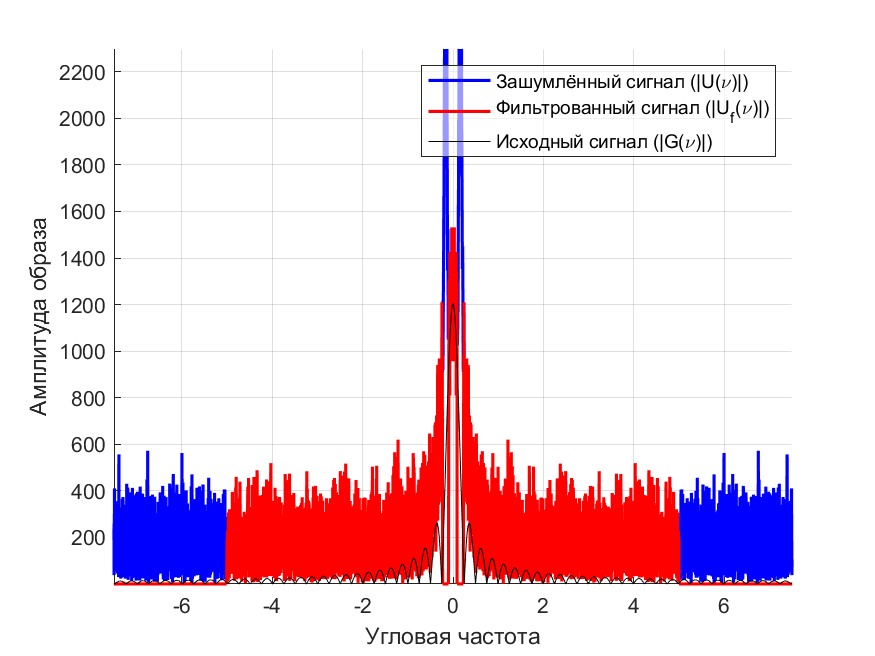
\includegraphics[width=\textwidth]{part2/1_8_1_Fourier_n.png}
        \caption{Модуль Фурье-образа, $b = 1, c = 8, d = 1, \nu_0 = 5$}
    \end{minipage}
\end{figure}\

Однако при таком преобразовании теряется слишком много низких частот, несущих полезную информацию. Попробуем сделать то же самое, изменив ещё и параметр $d$, к примеру, взяв $d = 10$:

\begin{figure}[H]
    \begin{minipage}{0.5\textwidth}
        \centering
        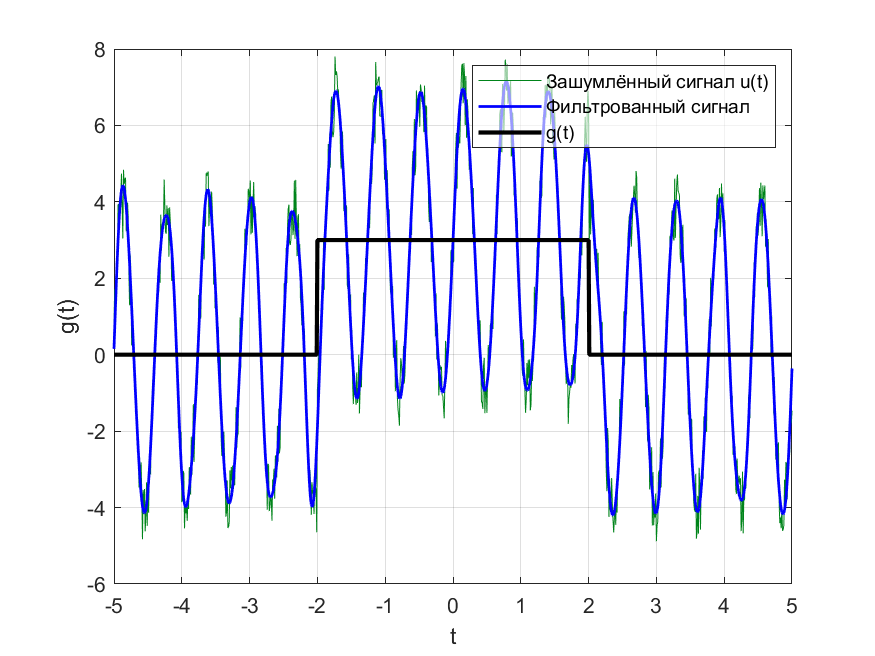
\includegraphics[width=\textwidth]{part2/1_4_10.png}
        \caption{$b = 1, c = 4, d = 10, \nu_0 = 5$}
    \end{minipage}    
    \begin{minipage}{0.5\textwidth}
        \centering
        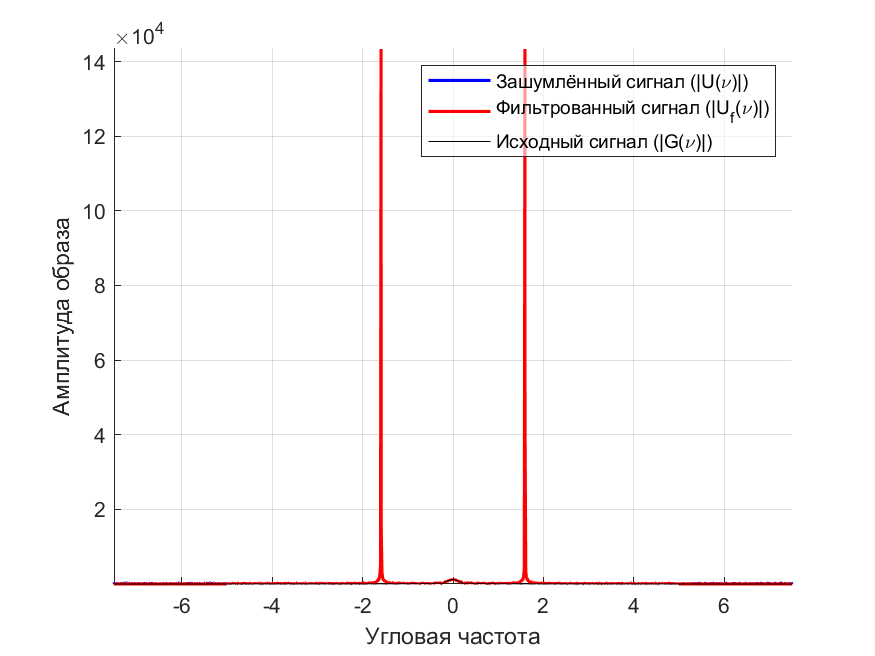
\includegraphics[width=\textwidth]{part2/1_4_10_Fourier.png}
        \caption{Модуль Фурье-образа, $b = 1, c = 4, d = 10, \nu_0 = 5$}
    \end{minipage}
\end{figure}\

\begin{figure}[H]
    \centering
    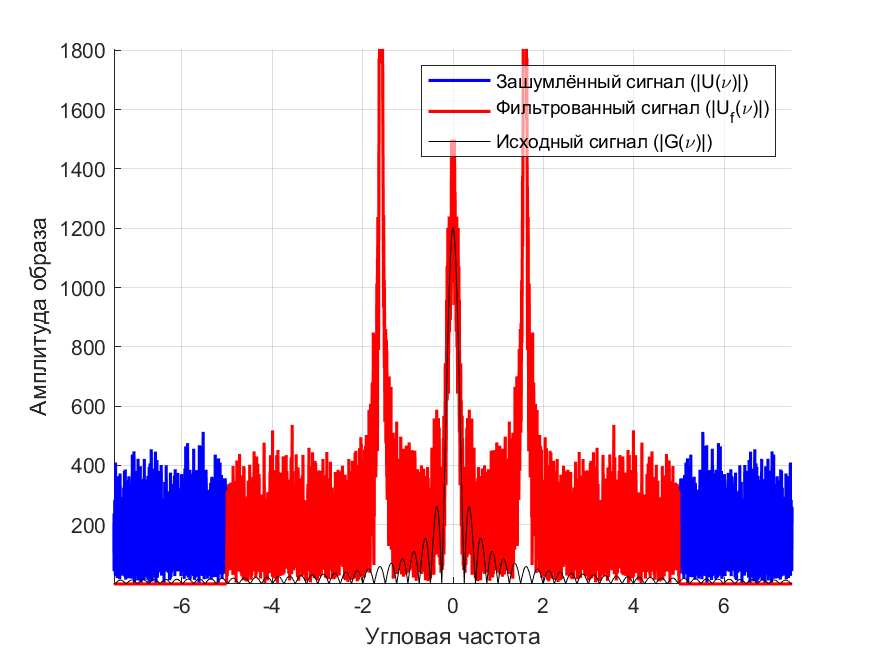
\includegraphics[width=0.5\linewidth]{part2/1_4_10_Fourier_scaled.png}
    \caption{Модуль Фурье-образа в приближении, $b = 1, c = 4, d = 10, \nu_0 = 5$}
\end{figure}\

В этом случае заметен пик на $\nu = 1.6$, и его уже безо всяких проблем можно будет обнулить. Сделаем это, вот результат:

\begin{figure}[H]
    \begin{minipage}{0.5\textwidth}
        \centering
        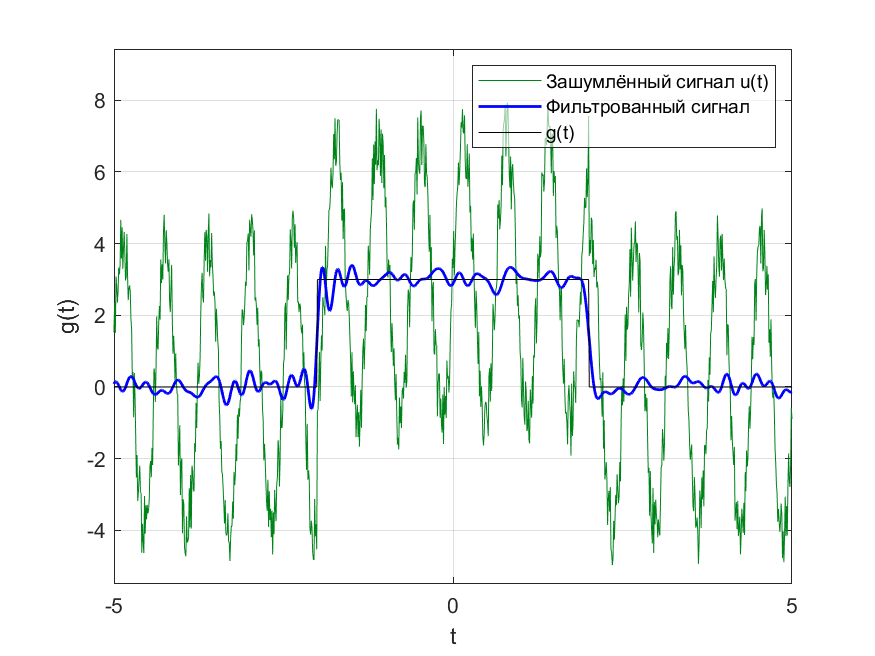
\includegraphics[width=\textwidth]{part2/1_4_10_n.png}
        \caption{$b = 1, c = 4, d = 10, \nu_0 = 5$}
    \end{minipage}    
    \begin{minipage}{0.5\textwidth}
        \centering
        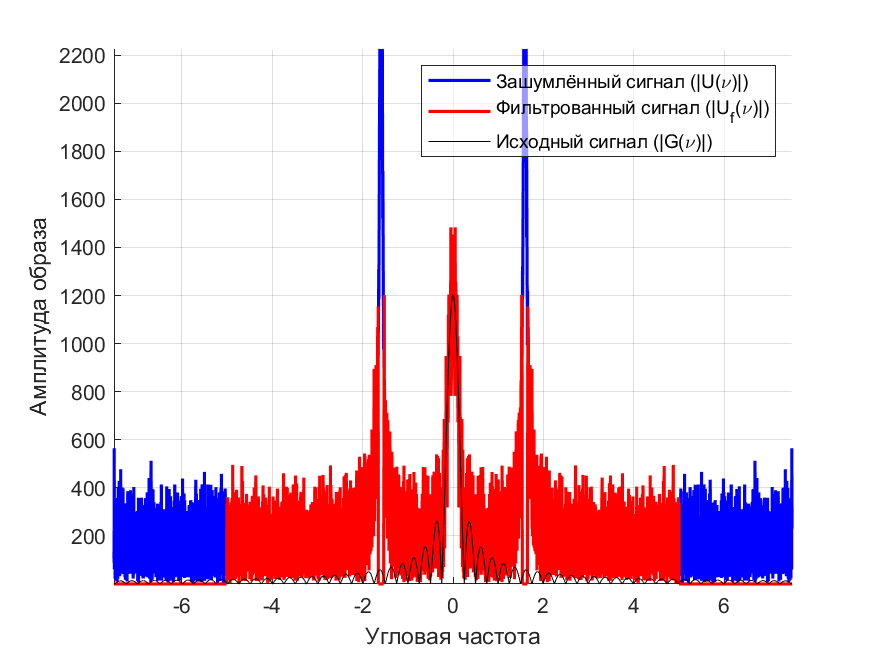
\includegraphics[width=\textwidth]{part2/1_4_10_Fourier_n.png}
        \caption{Модуль Фурье-образа, $b = 1, c = 4, d = 10, \nu_0 = 5$}
    \end{minipage}
\end{figure}\

Чудесным образом мы получили абсолютно тот же результат, что и с $c = 0$ --- остаётся только влияние шума, вызванного слагаемым $b \, \xi(t)$. То есть в теории, если бы помехи были только гармоническими (случай $b = 0$), мы могли бы полностью от них избавиться.

\subsubsection{Исследование влияния значения коэффициента $d$}\

В прошлом подпункте я немного затронул изменение этого коэффициента для сдвига пика образа зашумлённого сигнала, в этом же попытаюсь понять, как именно он влияет на вид помехи и эффективность фильтрации.\ 

Рассмотрим $d = 5$:

\begin{figure}[H]
    \begin{minipage}{0.5\textwidth}
        \centering
        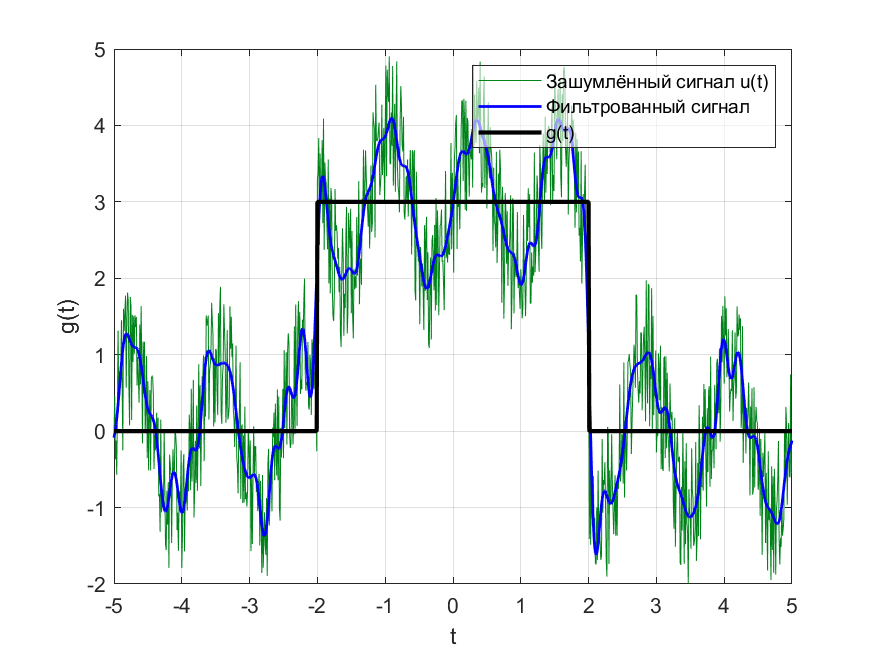
\includegraphics[width=\textwidth]{part2/1_1_5.png}
        \caption{$b = 1, c = 1, d = 5, \nu_0 = 5$}
    \end{minipage}    
    \begin{minipage}{0.5\textwidth}
        \centering
        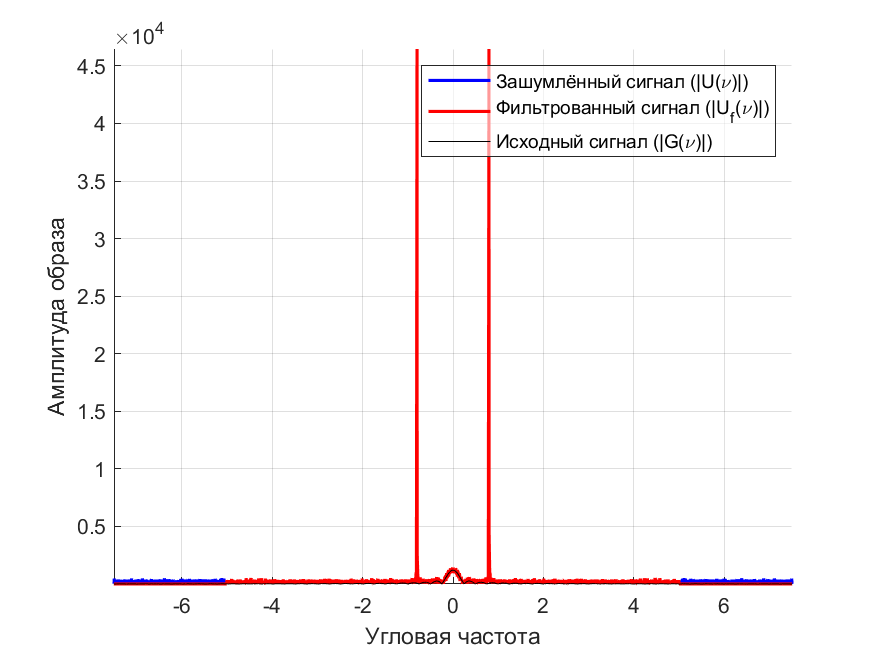
\includegraphics[width=\textwidth]{part2/1_1_5_Fourier.png}
        \caption{Модуль Фурье-образа, $b = 1, c = 1, d = 5, \nu_0 = 5$}
    \end{minipage}
\end{figure}\

\begin{figure}[H]
    \centering
    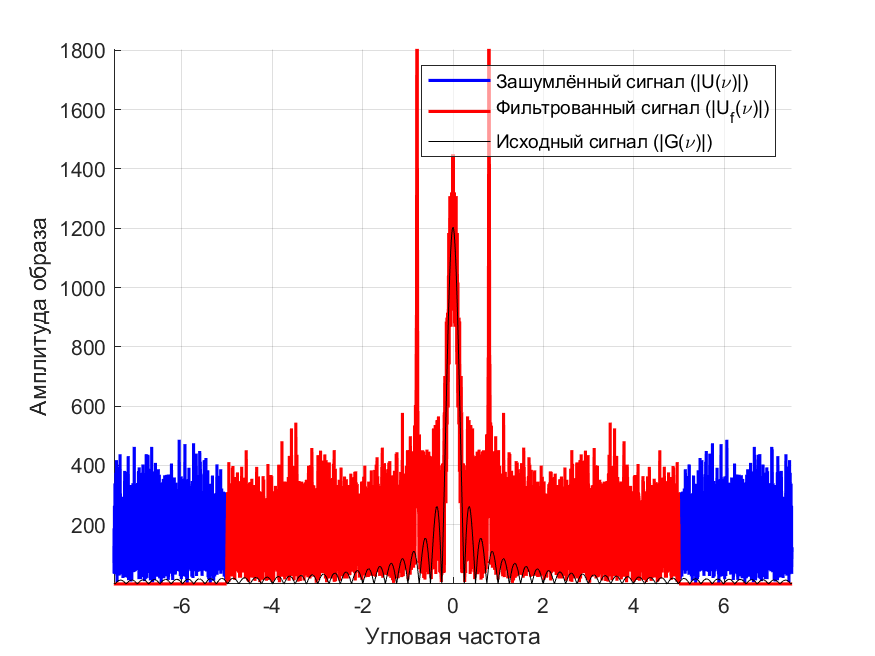
\includegraphics[width=0.5\linewidth]{part2/1_1_5_Fourier_scaled.png}
    \caption{Модуль Фурье-образа в приближении, $b = 1, c = 1, d = 5, \nu_0 = 5$}
\end{figure}\

Заметно, что увеличилось количество периодов синуса, охваченных графиком, продолжим увеличивать коэффициент, рассмотрим $d = 15$:

\begin{figure}[H]
    \begin{minipage}{0.5\textwidth}
        \centering
        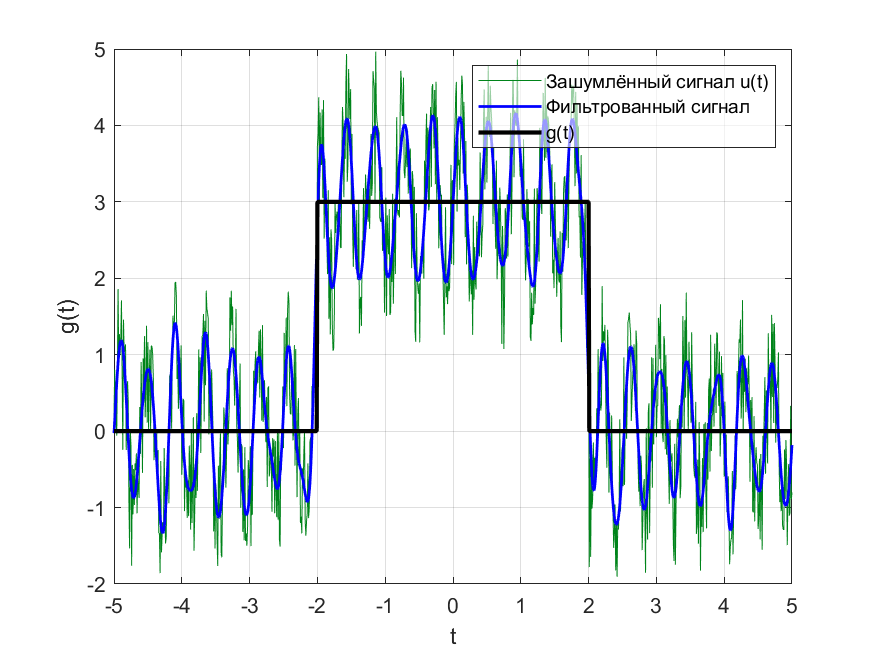
\includegraphics[width=\textwidth]{part2/1_1_15.png}
        \caption{$b = 1, c = 1, d = 15, \nu_0 = 5$}
    \end{minipage}    
    \begin{minipage}{0.5\textwidth}
        \centering
        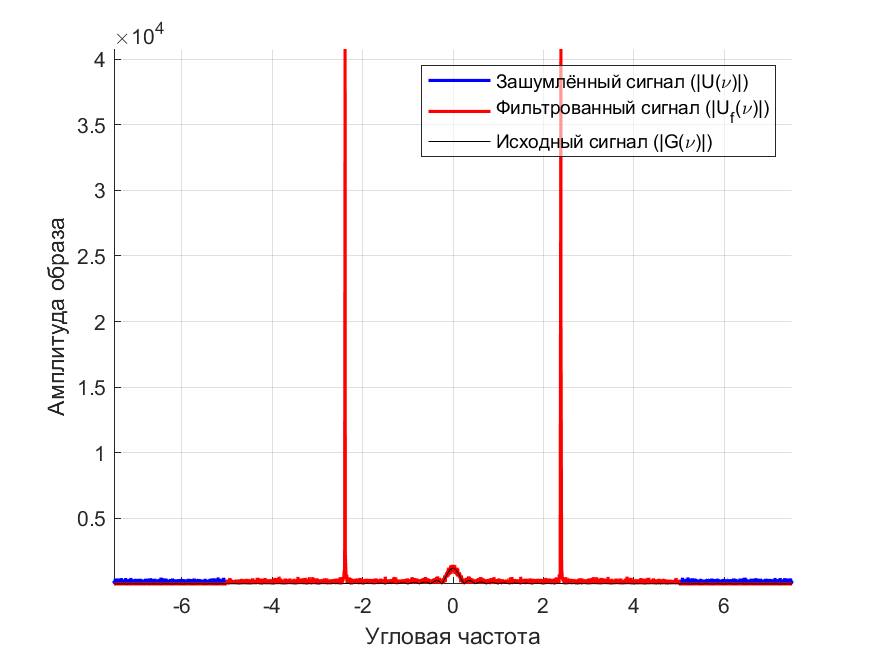
\includegraphics[width=\textwidth]{part2/1_1_15_Fourier.png}
        \caption{Модуль Фурье-образа, $b = 1, c = 1, d = 15, \nu_0 = 5$}
    \end{minipage}
\end{figure}\

\begin{figure}[H]
    \centering
    \includegraphics[width=0.5\linewidth]{part2/1_1_5_Fourier_scaled.png}
    \caption{Модуль Фурье-образа в приближении, $b = 1, c = 1, d = 15, \nu_0 = 5$}
\end{figure}\

Отсюда уже можно сделать вывод о влиянии коэффициента $d$ на вид помех --- чем он выше, тем меньше период колебаний, и, соответственно, больше частота колебаний. Исходя из графиков модулей образов же можно отметить, что при увеличении $d$ шум как бы сдвигается на более высокие частоты, что позволяет при больших значениях этого коэффициента и $b = 0$ восстанавливать сигнал фактически без потерь.

\subsubsection{Вывод}\

Сейчас я понимаю, как влияют на фильтрацию все рассмотренные параметры, а также понимаю, что сигнал с гармоническими помехами может быть обработан гораздо более эффективно, чем аналогичный со случайными помехами.

\subsection{Обработка низких частот?}\

Ещё в прошлом пункте при попытке работы с пиком около нуля я столкнулся с тем, что при обнулении пика потерял много исходных данных, и уже понимаю, что ни к чему хорошему это не приведёт. Для начала обнулим значения около ноля: $[-0.5, 0.5]$. Вот что получим:

\begin{figure}[H]
    \begin{minipage}{0.5\textwidth}
        \centering
        \includegraphics[width=\textwidth]{part3/1_1_1.png}
        \caption{$b = 1, c = 1, d = 1, \nu_0 = 0.5$}
    \end{minipage}    
    \begin{minipage}{0.5\textwidth}
        \centering
        \includegraphics[width=\textwidth]{part3/1_1_1_Fourier.png}
        \caption{Модуль Фурье-образа, $b = 1, c = 1, d = 1, \nu_0 = 0.5$}
    \end{minipage}
\end{figure}\

Уже тут берётся лишь малая часть полезного сигнала. Исключим его почти полностью, взяв промежуток побольше: $[-3, 3]$. Вот результат:

\begin{figure}[H]
    \begin{minipage}{0.5\textwidth}
        \centering
        \includegraphics[width=\textwidth]{part3/1_1_1_3.png}
        \caption{$b = 1, c = 1, d = 1, \nu_0 = 3$}
    \end{minipage}    
    \begin{minipage}{0.5\textwidth}
        \centering
        \includegraphics[width=\textwidth]{part3/1_1_1_Fourier_3.png}
        \caption{Модуль Фурье-образа, $b = 1, c = 1, d = 1, \nu_0 = 3$}
    \end{minipage}
\end{figure}\

Во все тяжкие. Обнулим весь образ сигнала:

\begin{figure}[H]
    \begin{minipage}{0.5\textwidth}
        \centering
        \includegraphics[width=\textwidth]{part3/1_1_1_inf.png}
        \caption{$b = 1, c = 1, d = 1, \nu_0 = \infty$}
    \end{minipage}    
    \begin{minipage}{0.5\textwidth}
        \centering
        \includegraphics[width=\textwidth]{part3/1_1_1_Fourier_inf.png}
        \caption{Модуль Фурье-образа, $b = 1, c = 1, d = 1, \nu_0 = \infty$}
    \end{minipage}
\end{figure}\

Ожидаемо, фильтрованный сигнал теперь тоже равен нулю на всей области своего определения.

\subsubsection{Вывод}\

Лучше не убирать низкие частоты, в них вся суть (разумеется, это не работает если сигнал существует на высоких частотах или если на низких частотах есть шумы, как это было с небольшим $d$ и с ненулевым $c$, тогда гармонический шум присутствовал на низкой частоте, но в этом случае убираются частоты не от 0 до $\nu_0$ (как это было в этом пункте), а от $\nu_0-\varepsilon$ до $\nu_0+\varepsilon$, что по сути другое).

\section{Фильтрация звука}\

Визуализация звукового сигнала (что по сути набор амплитуд) немного отличается от визуализации сигнала, заданного формулой, как было в предыдущем задании, и из-за этого пришлось изменить массив частот, для его правильного нахождения нужно задать массив значений в интервале $[-\frac{f}{2}, \frac{f}{2}]$ с шагом $\frac{f}{N}$, где $f$ --- частота дискретизации, а $N$ --- количество точек сигнала.\

Человеческий голос обычно звучит в диапазоне от 200 до 6000 Гц. С этого диапазона я и начал, постепенно корректируя рабочий диапазон. Шумы полностью перестали быть слышимы, когда я ограничил образ фильтрованного звукового сигнала с 300 до 5000 Гц, этот диапазон показался оптимальным. Соответственно такое условие и стало фильтром образа, все частоты ниже 300 и выше 5000 Гц были убраны, после чего получился наиболее чистый голос, хоть и немного ``плоский''. Вот получившиеся графики:\

\begin{figure}[H]
    \centering
    \includegraphics[width=0.5\linewidth]{ex2/sound.png}
    \caption{Сравнительные графики исходного и фильтрованного звукового сигнала}
\end{figure}

\begin{figure}[H]
    \begin{minipage}{0.5\textwidth}
        \centering
        \includegraphics[width=\textwidth]{ex2/snd_original_Fourier.png}
        \caption{График модуля Фурье-образа исходного звукового сигнала}
    \end{minipage}    
    \begin{minipage}{0.5\textwidth}
        \centering
        \includegraphics[width=\textwidth]{ex2/snd_filtered_Fourier.png}
        \caption{График модуля Фурье-образа фильтрованного звукового сигнала}
    \end{minipage}
\end{figure}\

В итоге после обработки остался только голос, лишние шумы были успешно убраны. 

\section{Выводы}\

В ходе проведённой работы я познакомился с прикладной частью преобразования Фурье, с различными помехами и видами их фильтрации, разобрался с влиянием коэффициентов зашумлённого сигнала на величину шумов, а также понял, что белый шум может помешать полной компенсации помех, в то время как гармонические помехи могут быть компенсированы полностью.

\end{document}